%%%%%%%%%%%%%%%%%%%%%%%%%%%%%%%%%%%%%%%%%%%%%%%%%%%%%%%%%%%%%%%%%%%%%%%%%%%%%
%
% api.tex
%
%
%%%%%%%%%%%%%%%%%%%%%%%%%%%%%%%%%%%%%%%%%%%%%%%%%%%%%%%%%%%%%%%%%%%%%%%%%%%%%


%%%%%%%%%%%%%%%%%%%%%%%%%%%%%%%%%%%%%%%%%%%%%%%%%%%%%%%%%%%%%%%%%%%%%%%%%%%%%
\chapt[chap:api]{GATE Embedded}
\markboth{GATE Embedded}{GATE Embedded}
%%%%%%%%%%%%%%%%%%%%%%%%%%%%%%%%%%%%%%%%%%%%%%%%%%%%%%%%%%%%%%%%%%%%%%%%%%%%%
\nnormalsize


%%%%%%%%%%%%%%%%%%%%%%%%%%%%%%%%%%%%%%%%%%%%%%%%%%%%%%%%%%%%%%%%%%%%%%%%%%%%%
\sect[sec:api:embed]{Quick Start with GATE Embedded}
%%%%%%%%%%%%%%%%%%%%%%%%%%%%%%%%%%%%%%%%%%%%%%%%%%%%%%%%%%%%%%%%%%%%%%%%%%%%%

\mbox{ }

Embedding GATE-based language processing in other applications using GATE
Embedded (the GATE API) is straightforward:

\begin{flushleft}
\sloppy
\begin{itemize}
\item add the GATE libraries to your application's classpath.
  \begin{itemize}
  \item if you use a build tool with dependency management, such
    as Maven or Gradle, add a dependency on the right version of
    \texttt{uk.ac.gate:gate-core} -- this is the recommended way
    to build against the GATE APIs.
  \item if you can't use a dependency manager, you can instead add
    all the JAR files from the \texttt{lib} directory of a GATE
    installation to your compile classpath in your build tool.
  \end{itemize}
\item initialise GATE with \texttt{gate.Gate.init();}
\item program to the framework API.
\end{itemize}
\fussy
\end{flushleft}
%
For example, this code will create the default ANNIE extraction system,
the same as the ``load ANNIE'' button in GATE Developer:
%
\begin{lstlisting}
  // initialise the GATE library
  Gate.init();

  // load the ANNIE plugin
  Plugin anniePlugin = new Plugin.Maven(
        "uk.ac.gate.plugins", "annie", gate.Main.version);
  Gate.getCreoleRegister().registerPlugin(anniePlugin);

  // load ANNIE application from inside the plugin
  SerialAnalyserController controller = (SerialAnalyserController)
    PersistenceManager.loadObjectFromUrl(new ResourceReference(
      anniePlugin, "resources/" + ANNIEConstants.DEFAULT_FILE)
        .toURL());
\end{lstlisting}
%
If you want to use resources from any plugins, you need to
load the plugins before calling \verb|createResource|:
\begin{lstlisting}
  Gate.init();

  // need Tools plugin for the Morphological analyser
  Gate.getCreoleRegister().registerPlugin(new Plugin.Maven(
    "uk.ac.gate.plugins", "tools", gate.Main.version));

  ...

  ProcessingResource morpher = (ProcessingResource)
    Factory.createResource("gate.creole.morph.Morph");
\end{lstlisting}
%
Instead of creating your processing resources individually using the
\texttt{Factory}, you can create your application in GATE Developer, save it using the
`save application state' option (see
Section~\ref{sec:developer:savestate}), and then load the saved state from
your code.  This will automatically reload any plugins that were
loaded when the state was saved, you do not need to load them
manually.
\begin{lstlisting}
  Gate.init();

  CorpusController controller = (CorpusController)
    PersistenceManager.loadObjectFromFile(new File("savedState.xgapp"));
\end{lstlisting}
There are many examples of using GATE Embedded available at:\\
\htlinkplain{http://gate.ac.uk/wiki/code-repository/}.


See Section~\ref{sec:gettingstarted:sysprop} for details of the system
properties GATE uses to find its configuration files.
%%%%%%%%%%%%%%%%%%%%%%%%%%%%%%%%%%%%%%%%%%%%%%%%%%%%%%%%%%%%%%%%%%%%%%%%%%%%%
\sect[sec:api:factory]{Resource Management in GATE Embedded}
%%%%%%%%%%%%%%%%%%%%%%%%%%%%%%%%%%%%%%%%%%%%%%%%%%%%%%%%%%%%%%%%%%%%%%%%%%%%%

% $ID$
As outlined earlier, GATE defines three different types of resources:
\begin{description}
\item[Language Resources]{: (\textbf{LRs}) entities that hold linguistic data.
}

\item[Processing Resources]{: (\textbf{PRs}) entities that process data.
}

\item[Visual Resources]{: (\textbf{VRs}) components used for building
graphical interfaces. }

\end{description}

These resources are collectively named \textbf{CREOLE}\footnote{CREOLE
stands for Collection of REusable Objects for Language Engineering} resources.

All CREOLE resources have some associated meta-data in the form of annotations
on the resource class and some of its methods.  The most important role of that
meta-data is to specify the set of parameters that a resource understands, which
of them are required and which not, if they have default values and what those
are. See Section \ref{sec:creole-model:config} for full details of the
configuration mechanism.

All resource types have creation-time parameters that are used during the
initialisation phase. Processing Resources also have run-time parameters
that get used during execution (see Section \ref{sec:api:pr} for more
details).

\textbf{Controllers} are used to define GATE applications and have the role of
controlling the execution flow (see Section \ref{sec:api:controllers} for
more details).

This section describes how to create and delete CREOLE resources as
objects in a running Java virtual machine. This process involves using
GATE's Factory class\footnote{Fully qualified
name: \tt{gate.Factory}}, and, in the case of LRs, may also involve
using a DataStore.

CREOLE resources are Java Beans; creation of a resource object
involves using a default constructor, then setting parameters on the
bean, then calling an {\tt init()} method. The Factory takes care of
all this, makes sure that the GATE Developer GUI is told about what is
happening (when GUI components exist at runtime), and also takes care
of restoring LRs from DataStores. \textbf{A programmer using GATE
Embedded should never call the constructor of a resource: always use
the Factory!}

Creating a resource involves providing the following information:
\begin{itemize}
\item \textbf{fully qualified class name} for the resource. This is the only
{\bf required} value. For all the rest, defaults will be used if actual values
are not provided.
\item values for the \textbf{creation time parameters}.$^\dagger\ $
\item initial values for \textbf{resource features}.$^\dagger\ $ For an
explanation on features see Section \ref{sec:api:features}.
\item a \textbf{name} for the new resource;
\end{itemize}

$^\dagger\ $ Parameters and features need to be provided in the form of a
GATE Feature Map which is essentially a java Map ({\tt java.util.Map})
implementation, see Section \ref{sec:api:features} for more details
on Feature Maps.

%\begin{minipage}{\textwidth}
%Here is an example that creates a GATE document:
%
%
%\begin{small}\begin{verbatim}
%URL u = new URL("http://gate.ac.uk/");
%FeatureMap params = Factory.newFeatureMap();
%params.put("sourceUrl", u);
%FeatureMap features = Factory.newFeatureMap();
%
%Document doc = (Document)
%  Factory.createResource("gate.corpora.DocumentImpl",
%                         params, features, "GATE Homepage");
%\end{verbatim}\end{small}
%
%\end{minipage}


%%%%%%%%%%%%%%%%%%%%%%%%%%%%%%%%%%%%%%%%%%%%%%%%%%%%%%%%%%%%%%%%%%%%%%%%%%%%%
%\subsect[sec:howto:instant]{Instantiating CREOLE Resources}
%%%%%%%%%%%%%%%%%%%%%%%%%%%%%%%%%%%%%%%%%%%%%%%%%%%%%%%%%%%%%%%%%%%%%%%%%%%%%

%This section describes how to create CREOLE resources as objects in a running
%Java virtual machine. This process involves using GATE's {\tt Factory} class,
%and, in the case of LRs, may also involve using a {\tt DataStore}.

%CREOLE resources are Java Beans; creation of a resource object
%involves using a default constructor, then setting parameters on the
%bean, then calling an {\tt init()} method\footnote{This method is not
%part of the beans spec.}. The Factory takes care of all this, makes
%sure that GATE Developer is told about what is happening (when GUI
%components exist at runtime), and also takes care of restoring LRs
%from DataStores. So a programmer using GATE Embedded should {\bf never
%call the constructor} of a resource: always use the Factory.

%The valid parameters for a resource are described in the resource's section
%of its {\tt creole.xml} file or in Java annotations on the resource class --
%see section \ref{sec:creole-model:config}.

Creating a resource via the Factory involves passing values for any
create-time parameters that require setting to the Factory's {\tt
createResource} method. If no parameters are passed, the defaults are used.
So, for example, the following code creates a default ANNIE part-of-speech
tagger:
%
\begin{lstlisting}
Gate.getCreoleRegister().registerPlugin(new Plugin.Maven(
      "uk.ac.gate.plugins", "annie", gate.Main.version));
FeatureMap params = Factory.newFeatureMap(); //empty map:default params
ProcessingResource tagger = (ProcessingResource)
  Factory.createResource("gate.creole.POSTagger", params);
\end{lstlisting}
%
Note that if the resource created here had any parameters that were both
mandatory and had no default value, the {\tt createResource} call would throw
an exception.  In the case of the POS tagger, all the required parameters have
default values so no \texttt{params} need to be passed in.

When creating a Document, however, the URL of the source for the document must be
provided\footnote{Alternatively a string giving the document source may be
provided.}. For example:
\begin{lstlisting}
URL u = new URL("https://gate.ac.uk/");
FeatureMap params = Factory.newFeatureMap();
params.put("sourceUrl", u);
Document doc = (Document)
  Factory.createResource("gate.corpora.DocumentImpl", params);
\end{lstlisting}
%
Note that the document created here is transient: when you quit the JVM the
document will no longer exist. If you want the document to be persistent, you need to
store it in a {\tt DataStore} (see Section~\ref{sec:api:corpora}).

Apart from {\tt createResource()} methods with different signatures, {\tt
Factory} also provides some shortcuts for common operations, listed in table
\ref{table:factory-op}.


\begin{table}[htbp]
\begin{small}
\begin{center}
\begin{tabular}{|p{.4\textwidth}|p{.4\textwidth}|}
\hline
\textbf{Method} & \textbf{Purpose}\\
\hline
{\tt {\bf newFeatureMap}()} & Creates a new Feature Map (as used in the
example above). \\
\hline
{\tt {\bf newDocument}(String content)} & Creates a new GATE Document starting
from a String value that will be used to generate the document content.\\
\hline
{\tt {\bf newDocument}(URL sourceUrl)} & Creates a new GATE Document
using the text pointed by an URL  to generate the document content.\\
\hline
{\tt {\bf newDocument}(URL sourceUrl, String encoding)} & Same as
above but allows the specification of an encoding to be used while
downloading the document content.\\
\hline
{\tt {\bf newCorpus}(String name)} & creates a new GATE Corpus with a specified
name.\\
\hline
\end{tabular}
\caption{Factory Operations}
\label{table:factory-op}
\end{center}
\end{small}
\end{table}



GATE maintains various data structures that allow the retrieval of loaded
resources. When a resource is no longer required, it needs to be removed from
those structures in order to remove all references to it, thus making it a
candidate for garbage collection. This is achieved using the {\tt
deleteResource(Resource res)} method on {\tt Factory}.

Simply removing all references to a resource from the user code will
{\bf NOT} be enough to make the resource collect-able. Not calling 
{\tt Factory.deleteResource()} {\bf will} lead to memory leaks!

%%%%%%%%%%%%%%%%%%%%%%%%%%%%%%%%%%%%%%%%%%%%%%%%%%%%%%%%%%%%%%%%%%%%%%%%%%%%%
\sect[sec:api:plugins]{Using CREOLE Plugins}
%%%%%%%%%%%%%%%%%%%%%%%%%%%%%%%%%%%%%%%%%%%%%%%%%%%%%%%%%%%%%%%%%%%%%%%%%%%%%

%When using GATE Embedded, the following API calls are relevant to working
%with plugins:

As shown in the examples above, in order to use a CREOLE resource the relevant
CREOLE plugin must be loaded. Processing Resources, Visual Resources and
Language Resources other than Document, Corpus and DataStore all require that the
appropriate plugin is first loaded. When using Document, Corpus or DataStore, you
do not need to first load a plugin. The following API calls listed in table
\ref{table:creole-calls} are relevant to working with CREOLE plugins.


\begin{table}[htbp]
\begin{small}
\begin{center}
\begin{tabular}{|p{.4\textwidth}|p{.4\textwidth}|}
\hline
\multicolumn{2}{|c|}{\textbf{Class \underline{gate.Gate}}}\\
\hline
\hline
\textbf{Method} & \textbf{Purpose}\\
\hline
{\tt public static void {\bf addKnownPlugin}(Plugin plugin)} & adds the plugin
to the list of known plugins.\\
\hline
{\tt public static void {\bf removeKnownPlugin}(Plugin plugin)} & tells the
system to `forget' about one previously known directory. If the specified plugin 
was loaded, it will be unloaded as well - i.e. all the metadata relating to 
resources defined by this plugin will be removed from memory.\\
\hline
{\tt public static void {\bf addAutoloadPlugin}(Plugin plugin)} & adds a new 
plugin to the list of plugins that are loaded automatically at start-up.\\
\hline
{\tt public static void {\bf removeAutoloadPlugin}(Plugin plugin)} & tells the 
system to remove a plugin from the list of plugins that are loaded 
automatically at system start-up. This will be reflected in the user's 
configuration data file.\\
\hline
\multicolumn{2}{|c|}{\textbf{Class \underline{gate.CreoleRegister}}}\\
\hline
\hline
{\tt public void {\bf registerPlugin}(Plugin plugin)} & loads a new
CREOLE plugin. The new plugin is added to the list of known plugins if not already
there.\\
\hline
{\tt public void {\bf unregisterPlugin}(Plugin plugin)} & unloads a loaded CREOLE
plugin.\\
\hline
\end{tabular}
\caption{Calls Relevant to CREOLE Plugins}
\label{table:creole-calls}
\end{center}
\end{small}
\end{table}

There are several different subclasses of \texttt{Plugin} that can be passed
to these methods.  The most common one is \texttt{Plugin.Maven}, as seen in the
examples above, which is a plugin that is a single JAR file specified via its
\texttt{group:artifact:version} ``coordinates'', and which is downloaded from a
Maven repository at runtime by GATE the first time the plugin is loaded.  The
vast majority of standard GATE plugins are of this type.  To load version 8.5
of the ANNIE plugin, for example, you would use:
\begin{lstlisting}
Gate.getCreoleRegister().registerPlugin(new Plugin.Maven(
      "uk.ac.gate.plugins", "annie", "8.5"));
\end{lstlisting}

In addition to Maven plugins, GATE still supports the style of plugins used in
GATE version 8.4.1 and earlier where the plugin is a directory on disk
which contains a \texttt{creole.xml} configuration file and optionally one or
more JAR files containing the compiled classes of the plugin's CREOLE
resources.  These plugins are represented by the class
\texttt{Plugin.Directory}, with a \texttt{URL} pointing to the directory that
contains the \texttt{creole.xml} file:
\begin{lstlisting}
Gate.getCreoleRegister().registerPlugin(new Plugin.Directory(
      new URL("file:/home/example/my-plugins/FishCounter/"));
\end{lstlisting}

Finally, if you are writing a GATE Embedded application and have a single
resource class that will only be used from your embedded code (and so does not
need to be distributed as a complete plugin), and all the configuration for
that resource is provided as Java annotations on the class, then it is possible
to register the class as a special type of \texttt{Plugin} called a
``component'':
\begin{lstlisting}
Gate.getCreoleRegister().registerPlugin(new Plugin.Component(
      MySpecialPurposePR.class));
\end{lstlisting}

Note that components cannot be registered this way in the developer GUI, and
cannot be included in saved application states (see
section~\ref{sec:api:persistent} below).

%%%%%%%%%%%%%%%%%%%%%%%%%%%%%%%%%%%%%%%%%%%%%%%%%%%%%%%%%%%%%%%%%%%%%%%%%%%%%
\sect[sec:api:lr]{Language Resources}
%%%%%%%%%%%%%%%%%%%%%%%%%%%%%%%%%%%%%%%%%%%%%%%%%%%%%%%%%%%%%%%%%%%%%%%%%%%%%

This section describes the
implementation of documents and corpora in GATE.

\subsect{GATE Documents}

Documents are modelled as content plus annotations (see Section
\ref{sec:api:annotations}) plus features (see Section
\ref{sec:api:features}).

The content of a document can be any implementation of the \linebreak\ {\tt
gate.DocumentContent} interface; the features are \verb!<!attribute,
value\verb!>! pairs stored a Feature Map. Attributes are String values while
the values can be any Java object.

The annotations are grouped in sets (see section \ref{sec:api:ann-sets}). A
document has a default (anonymous) annotations set and any number of named
annotations sets.

Documents are defined by the {\tt gate.Document} interface and there is also a
provided implementation:
\begin{description}
\item[{\tt \htlink{http://gate.ac.uk/gate/doc/javadoc/gate/corpora/DocumentImpl.html}{gate.corpora.DocumentImpl}}]: transient document. Can be stored
persistently through Java serialisation.
%
\end{description}

Main Document functions are presented in table \ref{table:document}.

\begin{table}[htbp]
\begin{small}
\begin{center}
\begin{tabular}{|p{.4\textwidth}|p{.4\textwidth}|}
\hline
\multicolumn{2}{|c|}{\textbf{Content Manipulation}}\\
\hline
\hline
\textbf{Method} & \textbf{Purpose}\\
\hline
{\tt DocumentContent {\bf getContent}()} & Gets the Document content. \\
\hline
{\tt void {\bf edit}(Long start, Long end, DocumentContent replacement)} &
Modifies the Document content.\\
\hline
{\tt void {\bf setContent}(DocumentContent newContent)} & Replaces the entire
content.\\
\hline
\multicolumn{2}{|c|}{\textbf{Annotations Manipulation}}\\
\hline
\hline
\textbf{Method} & \textbf{Purpose}\\
\hline
{\tt public AnnotationSet {\bf getAnnotations}()} & Returns the default annotation
set.\\
\hline
{\tt public AnnotationSet {\bf getAnnotations}(String name)} & Returns a {\em
named} annotation set.\\
\hline
{\tt public Map {\bf getNamedAnnotationSets}()} & Returns {\em all} the named
annotation sets.\\
\hline
{\tt void {\bf removeAnnotationSet}(String name)} & Removes a named
annotation set.\\
\hline
\multicolumn{2}{|c|}{\textbf{Input Output}}\\
\hline
\hline
{\tt String {\bf toXml}()} & Serialises the Document in XML format.\\
\hline
{\tt String {\bf toXml}(Set aSourceAnnotationSet, boolean includeFeatures)}
& Generates XML from a set of annotations only, trying to preserve the
original format of the file used to create the document.\\ 
\hline
\end{tabular}
\caption{{\tt gate.Document} methods.}
\label{table:document}
\end{center}
\end{small}
\end{table}


%%%%%%%%%%%%%%%%%%%%%%%%%%%%%%%%%%%%%%%%%%%%%%%%%%%%%%%%%%%%%%%%%%%%%%%%%%%%%
\subsect[sec:api:features]{Feature Maps}
%%%%%%%%%%%%%%%%%%%%%%%%%%%%%%%%%%%%%%%%%%%%%%%%%%%%%%%%%%%%%%%%%%%%%%%%%%%%%

All CREOLE resources as well as the {\em Controllers} and the annotations
can have attached meta-data in the form of {\em Feature Maps}.

A Feature Map is a Java Map (i.e. it implements the {\tt java.util.Map}
interface) and holds \verb!<!attribute-name, attribute-value\verb!>! pairs.
The attribute names are Strings while the values can be any Java Objects.

The use of non-{\em Serialisable} objects as values is strongly discouraged.

Feature Maps are created using the {\tt gate.Factory.newFeatureMap()}
method.

The actual implementation for FeatureMaps is provided by the \linebreak\ {\tt
gate.util.SimpleFeatureMapImpl} class.

Objects that have features in GATE implement the {\tt
gate.util.FeatureBearer} interface which has only the two accessor methods
for the object features: {\tt FeatureMap getFeatures()} and {\tt void
setFeatures(FeatureMap features)}.

\begin{minipage}{\textwidth}
{\b Getting a particular feature from an object}


\begin{lstlisting}
Object obj;
String featureName = "length";
if(obj instanceof FeatureBearer){
  FeatureMap features = ((FeatureBearer)obj).getFeatures();
  Object value = (features == null) ? null :
                                      features.get(featureName);
}
\end{lstlisting}

\end{minipage}

%%%%%%%%%%%%%%%%%%%%%%%%%%%%%%%%%%%%%%%%%%%%%%%%%%%%%%%%%%%%%%%%%%%%%%%%%%%%%
\subsect[sec:api:ann-sets]{Annotation Sets}
%%%%%%%%%%%%%%%%%%%%%%%%%%%%%%%%%%%%%%%%%%%%%%%%%%%%%%%%%%%%%%%%%%%%%%%%%%%%%


A GATE document can have one or more annotation layers --- an anonymous one,
(also called {\em default}), and as many {\em named} ones as necessary.

An annotation layer is organised as a \emph{Directed Acyclic Graph (DAG)} on
which the nodes are particular locations ---\emph{anchors}--- in the document content
and the arcs are made out of annotations reaching from the location indicated
by the start node to the one pointed by the end node (see Figure
\ref{fig:ann-graph} for an illustration). Because of the \emph{graph} metaphor,
the annotation layers are also called \emph{annotation graphs}.
In terms of Java objects, the annotation layers are represented using
the \emph{Set} paradigm as defined by the collections library and they are hence
named \emph{annotation sets}. The terms of annotation \emph{layer}, \emph{graph}
and \emph{set} are interchangeable and refer to the same concept when used in
this \thing{}.

\begin{figure}[htbp]
\begin{center}
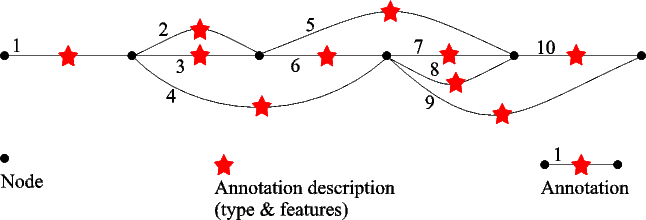
\includegraphics[scale=0.5]{annotationGraph.png}
\caption{The Annotation Graph model.}
\label{fig:ann-graph}
\end{center}
\end{figure}

An annotation set holds a number of annotations and maintains a series of
indices in order to provide fast access to the contained annotations.

The GATE Annotation Sets are defined by the {\tt gate.AnnotationSet}
interface and there is a default implementation provided:

\begin{description}
%
\item[{\tt \htlink{http://gate.ac.uk/gate/doc/javadoc/gate/annotation/AnnotationSetImpl.html}{gate.annotation.AnnotationSetImpl}}]
annotation set implementation used by transient documents.
\end{description}

The annotation sets are created by the document as required. The first time
a particular annotation set is requested from a document it will be
transparently created if it doesn't exist.

Tables \ref{table:annSet1} and \ref{table:annSet2} list the most used
Annotation Set functions.

\begin{table}[htbp]
\begin{small}
\begin{center}
\begin{tabular}{|p{.4\textwidth}|p{.4\textwidth}|}
\hline
\multicolumn{2}{|c|}{\textbf{Annotations Manipulation}}\\
\hline
\hline
\textbf{Method} & \textbf{Purpose}\\
\hline
{\tt Integer {\bf add}(Long start, Long end, String type, FeatureMap features)}
& Creates a new annotation between two offsets, adds it to this set and returns its id.\\
\hline
{\tt Integer {\bf add}(Node start, Node end, String type, FeatureMap
features)} & Creates a new annotation between two nodes, adds it to this
set and returns its id.\\
\hline
{\tt boolean {\bf remove}(Object o)} & Removes an annotation from this
set.\\
\hline

\multicolumn{2}{|c|}{\textbf{Nodes}}\\
\hline
\hline
\textbf{Method} & \textbf{Purpose}\\
\hline
{\tt Node {\bf firstNode}()} & Gets the node with the smallest offset.\\
\hline
{\tt Node {\bf lastNode}()} & Gets the node with the largest offset.\\
\hline
{\tt Node {\bf nextNode}(Node node)} & Get the first node that is relevant
for this annotation set and which has the offset larger than the one of the
node provided.\\
\hline
\multicolumn{2}{|c|}{\textbf{Set implementation}}\\
\hline
\hline
{\tt Iterator {\bf iterator}() } & \\
\hline
{\tt int {\bf size}()} & \\
\hline
\end{tabular}
\caption{{\tt gate.AnnotationSet} methods (general purpose).}
\label{table:annSet1}
\end{center}
\end{small}
\end{table}


\begin{table}[htbp]
\begin{center}
\begin{small}
\begin{tabular}{|p{.4\textwidth}|p{.4\textwidth}|}
\hline
\multicolumn{2}{|c|}{\textbf{Searching}}\\
\hline
\hline
{\tt AnnotationSet {\bf get}(Long offset)} & Select annotations by offset.
This returns the set of annotations whose start node is the least such that
it is greater than or equal to offset. If a positional index doesn't exist it
is created. If there are no nodes at or beyond the offset parameter then it
will return null.\\
\hline
{\tt AnnotationSet {\bf get}(Long startOffset, Long endOffset)} &
Select annotations by offset. This returns the set of annotations that
overlap totally or partially with the interval defined by the two provided
offsets. The result will include all the annotations that either:
\begin{itemize}
\item start before the start offset and end strictly after it
\item start at a position between the start and the end offsets
\end{itemize}\\
\hline
{\tt AnnotationSet {\bf get}(String type)} & Returns all annotations of the
specified type.\\
\hline
{\tt AnnotationSet {\bf get}(Set types)} & Returns all annotations of the
specified types.\\
\hline
{\tt AnnotationSet {\bf get}(String type, FeatureMap constraints)} & Selects
annotations by type and features.\\
\hline
{\tt Set {\bf getAllTypes}()} & Gets a set of java.lang.String objects
representing all the annotation types present in this annotation set.\\
\hline
{\tt AnnotationSet {\bf getContained}(Long startOffset, Long endOffset)} &
Select annotations contained within an interval, i.e.\\
\hline
{\tt AnnotationSet {\bf getCovering}(String neededType, Long startOffset,
Long endOffset)} &
Select annotations of the given type that completely span the range.\\
\hline
\end{tabular}
\caption{{\tt gate.AnnotationSet} methods (searching).}
\label{table:annSet2}
\end{small}
\end{center}
\end{table}

\begin{minipage}{\textwidth}
{\b Iterating from left to right over all annotations of a given
type}

\
\begin{lstlisting}
AnnotationSet annSet = ...;
String type = "Person";
//Get all person annotations
AnnotationSet persSet = annSet.get(type);
//Sort the annotations
List persList = new ArrayList(persSet);
Collections.sort(persList, new gate.util.OffsetComparator());
//Iterate
Iterator persIter = persList.iterator();
while(persIter.hasNext()){
...
}
\end{lstlisting}

\end{minipage}

%%%%%%%%%%%%%%%%%%%%%%%%%%%%%%%%%%%%%%%%%%%%%%%%%%%%%%%%%%%%%%%%%%%%%%%%%%%%%
\subsect[sec:api:annotations]{Annotations}
%%%%%%%%%%%%%%%%%%%%%%%%%%%%%%%%%%%%%%%%%%%%%%%%%%%%%%%%%%%%%%%%%%%%%%%%%%%%%

An \textbf{annotation} is a form of meta-data attached to a particular
section of document content. The connection between the annotation and the
content it refers to is made by means of two pointers that represent the
start and end locations of the covered content. An annotation must also have
a type (or a name) which is used to create classes of similar annotations,
usually linked together by their semantics.

An Annotation is defined by:
\begin{description}
\item[start node] a location in the document content defined by an offset.
\item[end  node] a location in the document content defined by an offset.
\item[type] a String value.
\item[features] (see Section~\ref{sec:api:features}).
\item[ID] an Integer value. All annotations IDs are unique inside an
annotation set.
\end{description}

In GATE Embedded, annotations are defined by the {\tt gate.Annotation}
interface and implemented by the {\tt gate.annotation.AnnotationImpl}
class.  Annotations exist only as members of annotation sets (see
Section~\ref{sec:api:ann-sets}) and they should not be directly created
by means of a constructor. Their creation should always be delegated
to the containing annotation set.

%%%%%%%%%%%%%%%%%%%%%%%%%%%%%%%%%%%%%%%%%%%%%%%%%%%%%%%%%%%%%%%%%%%%%%%%%%%%%
\subsect[sec:api:corpora]{GATE Corpora}
%%%%%%%%%%%%%%%%%%%%%%%%%%%%%%%%%%%%%%%%%%%%%%%%%%%%%%%%%%%%%%%%%%%%%%%%%%%%%

A corpus in GATE is a Java List (i.e. an implementation of {\tt
java.util.List}) of documents. GATE corpora are defined by the {\tt
gate.Corpus} interface and the following implementations are available:
\begin{description}
\item[{\tt gate.corpora.CorpusImpl}] used for transient corpora.
\item[{\tt gate.corpora.SerialCorpusImpl}] used for persistent corpora that
are stored in a serial datastore (i.e. as a directory in a file system).
\end{description}

Apart from implementation for the standard List methods, a Corpus also
implements the methods in table \ref{table:corpus}.

\begin{table}[htbp]
\begin{small}
\begin{center}
\begin{tabular}{|p{.4\textwidth}|p{.4\textwidth}|}
\hline
\textbf{Method} & \textbf{Purpose}\\
\hline
{\tt String {\bf getDocumentName}(int index)} & Gets the name of a document
in this corpus.\\
\hline
{\tt List {\bf getDocumentNames}()} & Gets the names of all the documents
in this corpus.\\
\hline
{\tt void {\bf populate}(URL directory, FileFilter filter, String encoding,
boolean recurseDirectories)} & Fills this corpus with documents created on
the fly from selected files in a directory. Uses a {\tt FileFilter} to
select which files will be used and which will be ignored. A simple file
filter based on extensions is provided in the Gate distribution ({\tt
gate.util.ExtensionFileFilter}).\\
{\tt void {\bf populate}(URL singleConcatenatedFile, String documentRootElement,
String encoding, int numberOfDocumentsToExtract, String documentNamePrefix, 
DocType documentType)} & Fills the provided corpus with documents extracted from
the provided single concatenated file. Uses the content between the start and 
end of the element as specified by {\tt documentRootElement} for each document.
The parameter {\tt documentType} specifies if the resulting files are html, xml
or of any other type. User can also restrict the number of documents to extract
by providing the relevant value for {\tt numberOfDocumentsToExtract} parameter.\\
\hline
\end{tabular}
\caption{{\tt gate.Corpus} methods.}
\label{table:corpus}
\end{center}
\end{small}
\end{table}

\begin{minipage}{\textwidth}

{\bf Creating a corpus from all XML files in a directory}


\begin{lstlisting}
Corpus corpus = Factory.newCorpus("My XML Files");
File directory = ...;
ExtensionFileFilter filter = new ExtensionFileFilter("XML files", "xml");
URL url = directory.toURL();
corpus.populate(url, filter, null, false);
\end{lstlisting}

\end{minipage}

{\bf Using a DataStore}

Assuming that you have a {\tt DataStore} already open called {\tt myDataStore},
this code will ask the datastore to take over persistence of your document, and
to synchronise the memory representation of the document with the disk storage:
\begin{small}\begin{verbatim}
Document persistentDoc = myDataStore.adopt(doc, mySecurity);
myDataStore.sync(persistentDoc);
\end{verbatim}\end{small}

%{\bf Security:}\\
%User access to the LRs is provided by a security mechanism of
%users and groups, similar to those on an operating system. When
%users create/save LRs into Oracle, they specify reading and
%writing access rights for users from their group and other users.
%For example, LRs created by one user/group can be made read-only
%to others, so they can use the data, but not modify it.
%The access modes are:
%\begin{itemize}
%\item
%others: read/none;
%\item
%group: modify/read/none;
%\item
%owner: modify/read.
%\end{itemize}
%If needed, ownership can be transferred from one user to another. Users,
%groups and LR permissions are
%administered in a special administration tool, by a privileged
%user. For more details see \Chapthing\ \ref{chap:security}.

When you want to restore a document (or other LR) from a datastore, you make
the same {\tt createResource} call to the Factory as for the creation of a
transient resource, but this time you tell it the datastore the resource
came from, and the ID of the resource in that datastore:
\begin{lstlisting}
  URL u = ....; // URL of a serial datastore directory
  SerialDataStore sds = new SerialDataStore(u.toString());
  sds.open();

  // getLrIds returns a list of LR Ids, so we get the first one
  Object lrId = sds.getLrIds("gate.corpora.DocumentImpl").get(0);

  // we need to tell the factory about the LR's ID in the data
  // store, and about which datastore it is in - we do this
  // via a feature map:
  FeatureMap features = Factory.newFeatureMap();
  features.put(DataStore.LR_ID_FEATURE_NAME, lrId);
  features.put(DataStore.DATASTORE_FEATURE_NAME, sds);

  // read the document back
  Document doc = (Document)
    Factory.createResource("gate.corpora.DocumentImpl", features);
\end{lstlisting}

%See the example code at \htlinkplain{http://gate.ac.uk/wiki/code-repository/}.


%%%%%%%%%%%%%%%%%%%%%%%%%%%%%%%%%%%%%%%%%%%%%%%%%%%%%%%%%%%%%%%%%%%%%%%%%%%%%
\sect[sec:api:pr]{Processing Resources}
%%%%%%%%%%%%%%%%%%%%%%%%%%%%%%%%%%%%%%%%%%%%%%%%%%%%%%%%%%%%%%%%%%%%%%%%%%%%%

Processing Resources ({\bf PRs}) represent entities that are primarily
algorithmic, such as parsers, generators or ngram modellers.

They are created using the GATE Factory in manner similar the
Language Resources. Besides the creation-time parameters they also
have a set of run-time parameters that are set by the system just
before executing them.

Analysers are a particular type of processing resources in the sense that
they always have a {\bf {\tt document}} and a {\bf {\tt corpus}} among their
run-time parameters.

The most used methods for Processing Resources are presented in table
\ref{table:pr}


\begin{table}[htbp]
\begin{small}
\begin{center}
\begin{tabular}{|p{.4\textwidth}|p{.4\textwidth}|}
\hline
\textbf{Method} & \textbf{Purpose}\\
\hline
{\tt void {\bf setParameterValue}(String paramaterName, Object
parameterValue)} & Sets the value for a specified parameter. {\small method
inherited from {\tt gate.Resource}}\\
\hline
{\tt void {\bf setParameterValues}(FeatureMap parameters)} & Sets the
values for more parameters in one step. {\small method inherited from {\tt
gate.Resource}}\\
\hline
{\tt Object {\bf getParameterValue}(String paramaterName)} & Gets the value
of a named parameter of this resource. {\small method inherited from {\tt
gate.Resource}}\\
\hline
{\tt Resource {\bf init}()} & Initialise this resource, and return it.
{\small method inherited from {\tt gate.Resource}}\\
\hline
{\tt void {\bf reInit}()} & Reinitialises the processing resource. After
calling this method the resource should be in the state it is after calling
init. If the resource depends on external resources (such as rules files)
then the resource will re-read those resources. If the data used to create
the resource has changed since the resource has been created then the
resource will change too after calling reInit().\\
\hline
{\tt void {\bf execute}()} & Starts the execution of this Processing
Resource.\\
\hline
{\tt void {\bf interrupt}()} & Notifies this PR that it should stop its
execution as soon as possible.\\
\hline
{\tt boolean {\bf isInterrupted}()} & Checks whether this PR has been
interrupted since the last time its Executable.execute() method was
called.\\
\hline
\end{tabular}
\caption{{\tt gate.ProcessingResource} methods.}
\label{table:pr}
\end{center}
\end{small}
\end{table}

%%%%%%%%%%%%%%%%%%%%%%%%%%%%%%%%%%%%%%%%%%%%%%%%%%%%%%%%%%%%%%%%%%%%%%%%%%%%%
\sect[sec:api:controllers]{Controllers}
%%%%%%%%%%%%%%%%%%%%%%%%%%%%%%%%%%%%%%%%%%%%%%%%%%%%%%%%%%%%%%%%%%%%%%%%%%%%%

Controllers are used to create GATE applications. A Controller handles a set of
Processing Resources and can execute them following a particular strategy.  GATE
provides a series of serial controllers (i.e. controllers that run their PRs in
sequence):

\begin{description}
\item[{\bf {\tt gate.creole.SerialController}:}] a serial controller that takes any
kind of PRs.
\item[{\bf {\tt gate.creole.SerialAnalyserController}:}] a serial controller that
only accepts Language Analysers as member PRs.
\item[{\bf {\tt gate.creole.ConditionalSerialController}:}] a serial controller
that accepts all types of PRs and that allows the inclusion or exclusion of
member PRs from the execution chain according to certain run-time conditions
(currently features on the document being processed are used).
\item[{\bf {\tt gate.creole.ConditionalSerialAnalyserController}:}] a serial
controller that only accepts Language Analysers and that allows the conditional
run of member PRs.
\item[{\bf {\tt gate.creole.RealtimeCorpusController}:}] a
{\tt SerialAnalyserController} that allows you to specify {\em graceful} and {\em timeout}
parameters (times in milliseconds).  If processing for a document takes longer than the 
amount of time specified for {\em graceful},  then the 
controller will attempt to gracefully end it by sending an interrupt 
request to it. If the {\em graceful} parameter is `-1' then no attempt to
gracefully end it is made. If processing takes longer than the amount of time 
specified for the {\em timeout} parameter, it 
will be forcibly terminated and the controller will move on to the next
document.  
The parameter {\em suppressExceptions} controls if time-outs and other 
exceptions will be suppressed or passed on to the caller: if this parameter
is set to `true', then any exception or a timeout will 
simply cause the controller to move on to the next document rather than failing
the entire corpus processing. If the parameter is set to `false' both 
time-outs and exceptions will be passed on as exceptions to the caller.
\end{description}

Additionally there is a {\em scriptable controller} provided by the Groovy
plugin.  See section~\ref{sec:api:groovy:controller} for details.

%\begin{minipage}{\textwidth}
{\bf Creating an ANNIE application and running it over a corpus}


\begin{lstlisting}
// load the ANNIE plugin
Plugin anniePlugin = new Plugin.Maven(
      "uk.ac.gate.plugins", "annie", gate.Main.version);
Gate.getCreoleRegister().registerPlugin(anniePlugin);

// create a serial analyser controller to run ANNIE with
SerialAnalyserController annieController =
 (SerialAnalyserController) Factory.createResource(
     "gate.creole.SerialAnalyserController",
     Factory.newFeatureMap(),
     Factory.newFeatureMap(), "ANNIE");

// load each PR as defined in ANNIEConstants
// Note this code is for demonstration purposes only,
// in practice if you want to load the ANNIE app you
// should use the PersistenceManager as shown at the
// start of this chapter
for(int i = 0; i < ANNIEConstants.PR_NAMES.length; i++) {
  // use default parameters
  FeatureMap params = Factory.newFeatureMap();
  ProcessingResource pr = (ProcessingResource)
      Factory.createResource(ANNIEConstants.PR_NAMES[i],
                             params);
  // add the PR to the pipeline controller
  annieController.add(pr);
} // for each ANNIE PR

// Tell ANNIE's controller about the corpus you want to run on
Corpus corpus = ...;
annieController.setCorpus(corpus);
// Run ANNIE
annieController.execute();
\end{lstlisting}

%\end{minipage}

%%%%%%%%%%%%%%%%%%%%%%%%%%%%%%%%%%%%%%%%%%%%%%%%%%%%%%%%%%%%%%%%%%%%%%%%%%%%%
\sect[sec:api:relations]{Modelling Relations between Annotations}
%%%%%%%%%%%%%%%%%%%%%%%%%%%%%%%%%%%%%%%%%%%%%%%%%%%%%%%%%%%%%%%%%%%%%%%%%%%%%

Most text processing tasks in GATE model metadata associated with text snippets
as annotations. In some cases, however, it is useful to to have another layer of
metadata, associated with the annotations themselves. One such case is the
modelling of relations between annotations. One typical example of relations
between annotation is that of co-reference. Two annotations of type {\tt Person}
may be referring to the same actual person; in this case the two annotations are
said to be co-referring.

Starting with version $7.1$, GATE Embedded supports the representation of
relations between annotations. A relation set is associated with, and accssed via,
an annotation set. All members of a relation must be either annotations from the
associated annotation set or other relations within the same set.
The classes supporting relations can be found in the \lstinline!gate.relations!
package.

A relation, as described by the \lstinline!gate.relations.Relation! interface,
is defined by the following values:
\begin{description}
\item[id] a unique ID that identifies the relation. IDs for both relations and
  annotations are generated from the same source, guaranteeing that not only is
  the ID unique among the relations, but also among all annotations from the
  same document.
\item[type] a String value describing the type of the relation (e.g. {\em
 'coref'} for co-reference relations).
\item[members] an \lstinline!int[]! array, containing the annotation IDs for the
  annotations referred to by the relation. Note that relations are not
  guaranteed to be symmetric, so the ordering in the members array is
  relevant.
\item[featureMap] a FeatureMap that, like with Annotations, allows the storing
  of an arbitary set of features for the relation.
\item[userData] an optional Serializable value, which can be used to associate
  any arbitrary data with a relation.
\end{description}

Relation sets are modelled by the \lstinline!gate.relations.RelationSet! class.
The principal API calls published by this class include:
\begin{itemize}
\item \lstinline!public Relation addRelation(String type, int... members)!\\
  Creates a new relation with the specified type and member annotations. Returns
  the newly created relation object.
\item \lstinline!public void addRelation(Relation rel)!\\
  Adds to this relation set an externally-created relation. This method is
  provided to support the use of custom implementations of the 
  \lstinline!gate.relations.Relation! interface.
\item \lstinline!public boolean deleteRelation(Relation relation)! \\
  Deletes the specified relation from this relation set. Any relations which
  include this relation as a member will also be deleted (recursively) to
  ensure the set remains internally consistent.
\item \lstinline!public Collection<Relation> get()!\\
  Returns all the relations within this set.
\item \lstinline!public Relation get(Integer id)!\\
  Returns the relation with the given ID.
\item \lstinline!public Collection<Relation> getRelations(String type)!\\
  Gets all relations with the specified type contained in this relation set.
\item \lstinline!public Collection<Relation> getRelations(int... members)!\\
  Gets relations by members. Gets all relations with have the specified members
  on the specified positions. The required members are represented as an
  \lstinline!int[]!, where each required annotation ID is placed on its required
  position. For unconstrained positions, the constant value
  \lstinline!gate.relations.RelationSet.ANY! should be used.
\item 
\lstinline!public Collection<Relation> getRelations(String type, int... members)!\\
  Gets all relations with the specified type and members.
\item \lstinline!public Collection<Relation> getReferencing(int id)!\\
  Gets all the relations which reference an annotation or relation with the
  specified ID.
\item \lstinline!public int getMaximumArity()!\\
  Gets the maximum arity (number of members) for all relations in this relation
  set.
\end{itemize}

Included next is a simple code snippet that illustrates the RelationSet API.
The function of the example code is to:
\begin{itemize}
  \item find all the {\tt Sentence} annotations inside a document;
  \item for each sentence, find all the contained {\tt Token} annotations;
  \item for each sentence and contained token, add a new relation named {\em
  contained} between the token and the sentence. 
\end{itemize}

\begin{lstlisting}
// get the document
Document doc = Factory.newDocument(
    new File("documents/file.xml").toURI().toURL());
// get the annotation set
AnnotationSet annSet = doc.getAnnotations();
// get the relations set
RelationSet relSet = annSet.getRelations();
// get all sentences
AnnotationSet sentences = annSet.get(
    ANNIEConstants.SENTENCE_ANNOTATION_TYPE);
for(Annotation sentence : sentences) {
  // get all the tokens
  AnnotationSet tokens = annSet.get(
      ANNIEConstants.TOKEN_ANNOTATION_TYPE,
      sentence.getStartNode().getOffset(),
      sentence.getEndNode().getOffset());
  for(Annotation token : tokens) {
    // for each sentence and token, add the contained relation
    relSet.addRelation("contained", 
        new int[] {token.getId(), sentence.getId()});
  }
}
\end{lstlisting}

%%%%%%%%%%%%%%%%%%%%%%%%%%%%%%%%%%%%%%%%%%%%%%%%%%%%%%%%%%%%%%%%%%%%%%%%%%%%%
\sect[sec:api:duplicate]{Duplicating a Resource}
%%%%%%%%%%%%%%%%%%%%%%%%%%%%%%%%%%%%%%%%%%%%%%%%%%%%%%%%%%%%%%%%%%%%%%%%%%%%%

Sometimes, particularly in a multi-threaded application, it is useful to be
able to create an independent copy of an existing PR, controller or LR.  The
obvious way to do this is to call {\tt createResource} again, passing the same
class name, parameters, features and name, and for many resources this will do
the right thing.  However there are some resources for which this may be
insufficient (e.g. controllers, which also need to duplicate their PRs), unsafe
(if a PR uses temporary files, for instance), or simply inefficient.  For
example for a large gazetteer this would involve loading a second copy of the
lists into memory and compiling them into a second identical state machine
representation, but a much more efficient way to achieve the same behaviour
would be to use a {\tt SharedDefaultGazetteer} (see
section~\ref{sec:gazetteers:shared}), which can re-use the existing state
machine.

The GATE {\tt Factory} provides a {\tt duplicate} method which takes an
existing resource instance and creates and returns an independent copy of the
resource.  By default it uses the algorithm described above, extracting the
parameter values from the template resource and calling {\tt createResource} to
create a duplicate (the actual algorithm is slightly more complicated than
this, see the following section).  However, if a particular resource type
knows of a better way to duplicate itself it can implement the
{\tt CustomDuplication} interface, and provide its own {\tt duplicate} method
which the factory will use instead of performing the default duplication
algorithm.  A caller who needs to duplicate an existing resource can simply
call {\tt Factory.duplicate} to obtain a copy, which will be constructed in the
appropriate way depending on the resource type.

Note that the duplicate object returned by {\tt Factory.duplicate} will
\emph{not necessarily} be of the same class as the original object.  However
the contract of {\tt Factory.duplicate} specifies that where the original
object implements any of a list of core GATE interfaces, the duplicate can be
assumed to implement the same ones -- if you duplicate a {\tt DefaultGazetteer}
the result may not be an instance of {\tt DefaultGazetteer} but it is
guaranteed to implement the {\tt Gazetteer} interface.

Full details of how to implement a custom duplicate method in your own resource
type can be found in the JavaDoc documentation for the
\htlink{http://gate.ac.uk/gate/doc/javadoc/gate/creole/CustomDuplication.html}%
{CustomDuplication interface} and the
\htlink{http://gate.ac.uk/gate/doc/javadoc/gate/Factory.html\#duplicate(gate.Resource)}%
{Factory.duplicate} method.

\subsect[sec:api:duplicate:sharable]{Sharable properties}

The \verb|@Sharable| annotation (in the \verb|gate.creole.metadata| package)
provides a way for a resource to mark JavaBean properties whose values should
be shared between a resource and its duplicates.  Typical examples of objects
that could be marked sharable include large or expensive-to-create data
structures that are created by a resource at init time and subsequently used in
a read-only fashion, a thread-safe cache of some sort, or state used to
create globally unique identifiers (such as an \verb|AtomicInteger| that is
incremented each time a new ID is required).  Clearly any ojects that are
shared between different resource instances must be accessed by all instances
in a way that is thread-safe or appropriately synchronized.

The sharable property must have the standard public getter and setter methods,
with the \verb|@Sharable| annotation applied to the setter\footnote{In the
common case where the getter/setter pair are simple accessors for a private
field whose name matches the Java Bean property name, the annotation may be
applied to the field rather than to the setter.}.  The same setter may be
marked both as a sharable property and as a \verb|@CreoleParameter| but
the two are not related -- sharable properties that are not parameters and
parameters that are not sharable are both allowed and both have uses in
different circumstances.  The use of sharable properties removes the need to
implement custom duplication in many simple cases.

The default duplication algorithm in full is thus as follows:
\begin{enumerate}
\item Extract the values of all init-time parameters from the original
  resource.
\item Recursively duplicate any of these values that are themselves GATE
  Resources, {\em except} for parameters that are marked as \verb|@Sharable|
  (i.e. parameters that are marked sharable are copied directly to the
  duplicate resource without being duplicated themselves).
\item Add to this parameter map any other sharable properties of the original
  resource (including those that are not parameters).
\item Extract the features of the original resource and recursively duplicate
  any values in this map that are themselves resources, as above.
\item Call \verb|Factory.createResource| passing the class name of the original
  resource, the duplicated/shared parameters and the duplicated features.
  \begin{itemize}
  \item this will result in a call to the new resource's \verb|init| method,
    with all sharable properties (parameters and non-parameters) populated with
    their values from the old resource.  The \verb|init| method must recognise
    this and adapt its behaviour appropriately, i.e. not re-creating sharable
    data structures that have already been injected.
  \end{itemize}
\item If the original resource is a PR, extract its runtime parameter values
  (except those that are marked as sharable, which have already been dealt with
  above), and recursively duplicate any resource values in the map.
\item Set the resulting runtime parameter values on the duplicate resource.
\end{enumerate}

The duplication process keeps track of any recursively-duplicated resources,
such that if the same original resource is used in several places (e.g.  when
duplicating a controller with several JAPE transducer PRs that all refer to the
same ontology LR in their runtime parameters) then the same duplicate
(ontology) will be used in the same places in the duplicated resource (i.e. all
the duplicate transducers will refer to the same ontology LR, which will be a
duplicate of the original one).

%%%%%%%%%%%%%%%%%%%%%%%%%%%%%%%%%%%%%%%%%%%%%%%%%%%%%%%%%%%%%%%%%%%%%%%%%%%%%
\sect[sec:api:persistent]{Persistent Applications}
%%%%%%%%%%%%%%%%%%%%%%%%%%%%%%%%%%%%%%%%%%%%%%%%%%%%%%%%%%%%%%%%%%%%%%%%%%%%%

GATE Embedded allows the persistent storage of applications in a
format based on XML serialisation. This is particularly useful for
applications management and distribution. A developer can save the
state of an application when he/she stops working on its design and
continue developing it in a next session. When the application reaches
maturity it can be deployed to the client site using the same method.

When an application (i.e. a {\em Controller}) is saved, GATE
will actually only save the values for the parameters used to create
the Processing Resources that are contained in the application. When
the application is reloaded, all the PRs will be re-created using the
saved parameters.

Many PRs use external resources (files) to define their behaviour and, in most
cases, these files are identified using URLs. During the saving process, all
the URLs are converted relative URLs based on the location of the
application file. This way, if the resources are packaged together with the
application file, the entire application can be reliably moved to a
different location.

API access to application saving and loading is provided by means of two
static methods on the {\tt gate.util.persistence.PersistenceManager} class,
listed in table \ref{table:save-load}.

\begin{table}[htbp]
\begin{small}
\begin{center}
\begin{tabular}{|p{.4\textwidth}|p{.4\textwidth}|}
\hline
\textbf{Method} & \textbf{Purpose}\\
\hline
{\tt public static void {\bf saveObjectToFile}(Object obj, File file)} & 
Saves the data needed to re-create the provided GATE object to the specified
file. The Object provided can be any type of Language or Processing Resource
or a Controller. The procedures may work for other types of objects as well
(e.g. it supports most Collection types).\\
\hline
{\tt public static Object {\bf loadObjectFromFile}(File file)} & Parses the
file specified (which needs to be a file created by the above method) and
creates the necessary object(s) as specified by the data in the file.
Returns the root of the object tree.\\
\hline
\end{tabular}
\caption{Application Saving and Loading}
\label{table:save-load}
\end{center}
\end{small}
\end{table}


%\begin{minipage}{\textwidth}
{\b Saving and loading a GATE application}


\begin{lstlisting}
//Where to save the application?
File file = ...;
//What to save?
Controller theApplication = ...;

//save
gate.util.persistence.PersistenceManager.
          saveObjectToFile(theApplication, file);
//delete the application
Factory.deleteResource(theApplication);
theApplication = null;

[...]
//load the application back
theApplication = gate.util.persistence.PersistenceManager.
                 loadObjectFromFile(file);
\end{lstlisting}

%\end{minipage}

%%%%%%%%%%%%%%%%%%%%%%%%%%%%%%%%%%%%%%%%%%%%%%%%%%%%%%%%%%%%%%%%%%%%%%%%%%%%%
\sect{Ontologies}
%%%%%%%%%%%%%%%%%%%%%%%%%%%%%%%%%%%%%%%%%%%%%%%%%%%%%%%%%%%%%%%%%%%%%%%%%%%%%

Starting from GATE version {\tt 3.1}, support for ontologies has been added.
Ontologies are nominally Language Resources but are quite different from
documents and corpora and are detailed in chapter~\ref{chap:ontologies}.

Classes related to ontologies are to be found in the {\tt gate.creole.ontology}
package and its sub-packages. The top level package defines an abstract API for
working with ontologies while the sub-packages contain concrete implementations.
A client program should only use the classes and methods defined in the 
API and never any of the classes or methods from the implementation packages.

The entry point to the ontology API is the {\tt gate.creole.ontology.Ontology}
interface which is the base interface for all concrete implementations. It
provides methods for accessing the class hierarchy, listing the instances and the
properties.

Ontology implementations are available through plugins. Before an ontology
language resource can be created using the \texttt{gate.Factory} and before
any of the classes and methods in the API can be used, one of the implementing
ontology plugins must be loaded. For details see chapter~\ref{chap:ontologies}.

%%%%%%%%%%%%%%%%%%%%%%%%%%%%%%%%%%%%%%%%%%%%%%%%%%%%%%%%%%%%%%%%%%%%%%%%%%%%%
\sect[sec:api:schemas]{Creating a New Annotation Schema}
%%%%%%%%%%%%%%%%%%%%%%%%%%%%%%%%%%%%%%%%%%%%%%%%%%%%%%%%%%%%%%%%%%%%%%%%%%%%%

An annotation schema (see Section~\ref{sec:developer:schemaannotationeditor}) can
be brought inside GATE through the creole.xml file. By using the AUTOINSTANCE
element, one can create instances of resources defined in creole.xml. The
gate.creole.AnnotationSchema (which is the Java representation of an annotation
schema file) initializes with some predefined annotation definitions (annotation
schemas) as specified by the GATE team.

{\em Example from GATE's internal creole.xml (in
  {\tt src/gate/resources/creole}):}

\small
\begin{small}\begin{verbatim}
<!-- Annotation schema -->
<RESOURCE>
  <NAME>Annotation schema</NAME>
  <CLASS>gate.creole.AnnotationSchema</CLASS>
  <COMMENT>An annotation type and its features</COMMENT>
  <PARAMETER NAME="xmlFileUrl" COMMENT="The url to the definition file"
    SUFFIXES="xml;xsd">java.net.URL</PARAMETER>
  <AUTOINSTANCE>
    <PARAM NAME ="xmlFileUrl" VALUE="schema/AddressSchema.xml" />
  </AUTOINSTANCE>
  <AUTOINSTANCE>
    <PARAM NAME ="xmlFileUrl" VALUE="schema/DateSchema.xml" />
  </AUTOINSTANCE>
  <AUTOINSTANCE>
    <PARAM NAME ="xmlFileUrl" VALUE="schema/FacilitySchema.xml" />
  </AUTOINSTANCE>
  <!-- etc. -->
</RESOURCE>
\end{verbatim}\end{small}
\nnormalsize

In order to create a gate.creole.AnnotationSchema object from a
schema annotation file, one must use the gate.Factory class;

\begin{lstlisting}
FeatureMap params = new FeatureMap();\\
param.put("xmlFileUrl",annotSchemaFile.toURL());\\
AnnotationSchema annotSchema = \\
Factory.createResurce("gate.creole.AnnotationSchema", params);
\end{lstlisting}

\noindent{\bf Note:} All the elements and their values must be written
in lower case, as XML is defined as case sensitive and the parser used
for XML Schema inside GATE searches is case sensitive.

In order to be able to write XML Schema definitions, the ones defined in
GATE (resources/creole/schema) can be used as a model, or the user can
have a look at {\em http://www.w3.org/2000/10/XMLSchema} for a
proper description of the semantics of the elements used.

Some examples of annotation schemas are given in Section \ref{sec:corpora:schemas}.

%%%%%%%%%%%%%%%%%%%%%%%%%%%%%%%%%%%%%%%%%%%%%%%%%%%%%%%%%%%%%%%%%%%%%%%%%%%%%
\sect[sec:api:bootstrap]{Creating a New CREOLE Resource}
%%%%%%%%%%%%%%%%%%%%%%%%%%%%%%%%%%%%%%%%%%%%%%%%%%%%%%%%%%%%%%%%%%%%%%%%%%%%%

%CREOLE resources are Java Beans (see \Chapthing\ \ref{chap:creole-model}).
%They come in three types: Language Resource, Processing Resource and Visual
%Resource (see \Chapthing\ \ref{chap:intro} Section \ref{sec:intro:developing}).

To create a new resource you need to:

%
\begin{itemize}
\item
write a Java class that implements GATE's beans model;
\item
annotate the class with the necessary CREOLE metadata;
\item
compile the class, and any others that it uses, into a Java Archive (JAR)
file, including a creole.xml file to identify the JAR as a plugin;
\item
tell GATE how to find the JAR.
\end{itemize}
%
The recommended way to build GATE plugins from version 8.5 onwards is to use
the Apache Maven build tool.  A JAR file requires certain specific contents in
order to be a valid GATE plugin, and GATE provides tools to automate the
creation of these as part of a Maven build.  For best results you should use
Maven 3.5.2 or later.

GATE provides a Maven \emph{archetype} to create the skeleton of a new plugin
including an example \texttt{AbstractLanguageAnalyser} processing resource you
can use as a starting point for your own code.
To create a new plugin project from the archetype, run the following Maven
command (which has been split over several lines for clarity, but should be run
as a single command):
\begin{verbatim}
mvn archetype:generate -DarchetypeGroupId=uk.ac.gate \
                       -DarchetypeArtifactId=gate-pr-archetype \
                       -DarchetypeVersion=8.5
\end{verbatim}
Replace ``8.5'' with the version of \texttt{gate-core} that you wish to depend
on.  You will be prompted for several values by Maven:
\begin{description}
\item[groupId] the group ID to use in the generated project POM. In Maven terms
  a ``group'' is a set of related JARs maintained and released by the same
  developer or group -- conventionally this is based on the same convention as
  Java \texttt{package} names, using a reversed form of a DNS domain you own.
  You can use any value you like here, except that you should \emph{not} use
  a group ID starting \texttt{uk.ac.gate}, as that is reserved for core plugins
  from the GATE team.
\item[artifactId] the artifact ID for the generated project POM -- this will be
  used as the directory name for the new project on disk and as the first part
  of the name of the final JAR file.
\item[version] the initial version number for your new plugin -- this should
  always end with \verb!-SNAPSHOT! in capital letters, which is a Maven
  convention denoting work-in-progress code where the same version number can
  refer to different JAR files over time.  The Maven dependency mechanism
  assumes that \emph{only} \verb!-SNAPSHOT! versions can ever change, and
  JAR files for non-SNAPSHOT versions are immutable and can be cached forever.
\item[package] the Java package name.  Often this is the same as the group ID
  but this is not strictly required.
\item[prClass] the class name of the PR class to generate -- this must be a
  valid Java identifier.
\item[prName] the name of the PR as it will appear to users in the GATE
  Developer GUI (e.g. in the ``new processing resource'' popup menu).
\end{description}

Alternatively you can specify any of these values as extra \verb!-D! options to
\verb!archetype:generate!, e.g. \verb!-DprClass=GoldfishTagger!.

The archetype will create a new directory named after the \texttt{artifactId},
containing a few files:
\begin{description}
\item[pom.xml] the Maven project descriptor controlling the build process
\item[src/main/java/\emph{package}/\emph{prClass}.java] the PR Java class.
\item[src/main/resources/creole.xml] the \emph{plugin descriptor} that
  identifies this project as a GATE plugin.
\item[src/main/resources/resources] a directory into which you should put any
  resource files that your PR requires (e.g. configuration files, JAPE
  grammars, etc.).  The doubled ``resources'' is deliberate --
  \verb!src/main/resources! is the Maven conventional location for non-Java
  files that should be packaged in the JAR, and GATE requires a folder called
  \verb!resources! inside that.
\item[src/test] some simple tests.
\end{description}

The generated Java class in \texttt{src/main/java} contains some basic CREOLE
metadata and an example of how you can configure parameters, and some
boilerplate initialization and execution code that you can modify to your
requirements.

There is an alternative archetype available called
\texttt{gate-plugin-archetype}, which creates the Maven project structure, POM
file and creole.xml but not the example Java class.  This is useful if you
already have an existing CREOLE plugin from an earlier version of GATE that you
want to convert to the Maven style.  The process is exactly the same as
described above, use the same \texttt{mvn archetype:generate} call as before
but with \verb!-DarchetypeArtifactId=gate-plugin-archetype!.

\subsection*{Dependencies}

If you need to use other Java libraries in your PR code you should declare them
in the \verb!<dependencies>! block of the \texttt{pom.xml}.  You can use
\htlinkplain{https://search.maven.org} to find the appropriate XML snippet for
each dependency.

If your plugin requires another GATE plugin to operate (for
example if it needs to internally create a JAPE transducer PR) then you
should declare a dependency on the relevant plugin in
\texttt{src/main/resources/creole.xml} and GATE will ensure that the other
plugin is always loaded before this one, and that this plugin is unloaded
whenever the other one is unloaded.

If your plugin has a \emph{compile-time} dependency on another plugin then you
will also need to declare this in \texttt{pom.xml} as well as in
\texttt{creole.xml} -- the pom dependency should use ``provided'' scope:
\begin{verbatim}
<dependency>
  <groupId>uk.ac.gate.plugins</groupId>
  <artifactId>annie</artifactId>
  <version>8.5</version>
  <scope>provided</scope>
</dependency>
\end{verbatim}
%
Note that such dependencies are very rarely required, typically only if you
need to write a PR class in one plugin that \texttt{extends} (in the Java
sense) a PR defined in another plugin.  If you simply need to \emph{run}
another plugin's PR as part of yours then the \texttt{creole.xml} dependency is
sufficient as you would create and use the PR via the \texttt{Factory} in the
normal way.
\begin{lstlisting}
// here we assume \texttt{grammarLocation} is declared as a \texttt{@CreoleParameter}
// of this PR and is of type \texttt{ResourceReference}
FeatureMap params = Utils.featureMap("grammarUrl", grammarLocation);
LanguageAnalyser jape = Factory.createResource(
      "gate.creole.Transducer", params);
\end{lstlisting}

%%%%%%%%%%%%%%%%%%%%%%%%%%%%%%%%%%%%%%%%%%%%%%%%%%%%%%%%%%%%%%%%%%%%%%%%%%%%%
\sect[sec:api:format]{Adding Support for a New Document Format}
%%%%%%%%%%%%%%%%%%%%%%%%%%%%%%%%%%%%%%%%%%%%%%%%%%%%%%%%%%%%%%%%%%%%%%%%%%%%%

In order to add a new document format, one needs to
extend the {\tt gate.DocumentFormat} class and to implement an
abstract method called:

\begin{lstlisting}
public void unpackMarkup(Document doc) throws
 DocumentFormatException
\end{lstlisting} 
 
This method is supposed to implement the functionality of each format
reader and to create annotations on the document. Finally the
document's old content will be replaced with a new one containing only
the text between markups.
% (see the GATE Embedded documentation for more
%details on this method functionality).

If one needs to add a new textual reader will extend the
gate.corpora.TextualDocumentFormat and override the {\tt
unpackMarkup(doc)} method.

This class needs to be implemented under the Java bean
specifications because it will be instantiated by GATE using {\tt
Factory.createResource()} method.

The {\tt init()} method that one needs to add and implement is
very important because in here the reader defines its means to be
selected successfully by GATE. What one needs to do is to add some
specific information into certain static maps defined in {\tt
DocumentFormat} class, that will be used at reader detection time.

After that, a definition of the reader will be placed into the
one's creole.xml file and the reader will be available to GATE.

We present for the rest of the section a complete three step
example of adding such a reader. The reader we describe in here is
an XML reader.

{\bf Step 1}

Create a new class called {\tt XmlDocumentFormat} that extends\\
{\tt gate.corpora.TextualDocumentFormat}.

{\bf Step 2}

Implement the {\tt unpackMarkup(Document doc)} which performs the
required functionality for the reader. Add XML detection means in
init() method:

\small
\begin{lstlisting}
public Resource init() throws ResourceInstantiationException{
  // Register XML mime type
  MimeType mime = new MimeType("text","xml");
  // Register the class handler for this mime type
  mimeString2ClassHandlerMap.put(mime.getType()+ "/" + mime.getSubtype(),
                                                             this);
  // Register the mime type with mine string
  mimeString2mimeTypeMap.put(mime.getType() + "/" + mime.getSubtype(),
                                                             mime);
  // Register file suffixes for this mime type
  suffixes2mimeTypeMap.put("xml",mime);
  suffixes2mimeTypeMap.put("xhtm",mime);
  suffixes2mimeTypeMap.put("xhtml",mime);
  // Register magic numbers for this mime type
  magic2mimeTypeMap.put("<?xml",mime);
  // Set the mimeType for this language resource
  setMimeType(mime);
  return this;
}// init()
\end{lstlisting}
\nnormalsize

More details about the information from those maps can be found in
Section \ref{sec:corpora:detecting-reader}

 {\bf Step 3}

Add the following creole definition in the creole.xml document.
\small
\begin{verbatim}
    <RESOURCE>
      <NAME>My XML Document Format</NAME>
      <CLASS>mypackage.XmlDocumentFormat</CLASS>
      <AUTOINSTANCE/>
      <PRIVATE/>
    </RESOURCE>
\end{verbatim}
\nnormalsize

More information on the operation of GATE's document format analysers may be
found in Section~\ref{sec:corpora:formats}.


%%%%%%%%%%%%%%%%%%%%%%%%%%%%%%%%%%%%%%%%%%%%%%%%%%%%%%%%%%%%%%%%%%%%%%%%%%%%%
\sect[sec:api:multithread]{Using GATE Embedded in a Multithreaded Environment}
%%%%%%%%%%%%%%%%%%%%%%%%%%%%%%%%%%%%%%%%%%%%%%%%%%%%%%%%%%%%%%%%%%%%%%%%%%%%%

GATE Embedded can be used in multithreaded applications, so long as
you observe a few restrictions.  First, you must initialise GATE by
calling \texttt{Gate.init()} {\em exactly once} in your application,
typically in the application startup phase before any concurrent
processing threads are started.

Secondly, you must not make calls that affect the global state of GATE (e.g.
loading or unloading plugins) in more than one thread at a time.  Again, you
would typically load all the plugins your application requires at
initialisation time.  It is safe to create {\em instances} of resources in
multiple threads concurrently.

Thirdly, it is important to note that individual GATE processing
resources, language resources and controllers are by design {\it not} thread
safe -- it is not possible to use a single instance of a controller/PR/LR in
multiple threads at the same time -- but for a well written resource it should
be possible to use several different instances of the same resource at once,
each in a different thread.  When writing your own resource classes you should
bear the following in mind, to ensure that your resource will be useable in
this way.
%
\begin{itemize}
\item Avoid static data.  Where possible, you should avoid using static fields
in your class, and you should try and take all configuration data via the
CREOLE parameters you declare in your creole.xml file.  System properties may
be appropriate for truly static configuration, such as the location of an
external executable, but even then it is generally better to stick to CREOLE
parameters -- a user may wish to use two different instances of your PR, each
talking to a different executable.
\item Read parameters at the correct time.  Init-time parameters should be read
in the \texttt{init()} (and \texttt{reInit()}) method, and for processing
resources runtime parameters should be read at each \texttt{execute()}.
\item Use temporary files correctly.  If your resource makes use of external
temporary files you should create them using \texttt{File.createTempFile()} at
\texttt{init} or \texttt{execute} time, as appropriate.  Do not use hardcoded
file names for temporary files.
\item If there are objects that can be shared between different instances of
your resource, make sure these objects are accessed either read-only, or in a
thread-safe way.  In particular you must be very careful if your resource can
take other resource instances as init or runtime parameters (e.g. the Flexible
Gazetteer, Section~\ref{sec:gazetteers:flexgazetteer}).
\end{itemize}

Of course, if you are writing a PR that is simply a wrapper around an external
library that imposes these kinds of limitations there is only so much you can
do.  If your resource cannot be made safe you should {\em document this fact
clearly}.

All the standard ANNIE PRs are safe when independent instances are used in
different threads concurrently, as are the standard transient document,
transient corpus and controller classes.  A typical pattern of development for
a multithreaded GATE-based application is:

\begin{itemize}
\item Develop your GATE processing pipeline in GATE Developer.
\item Save your pipeline as a \texttt{.gapp} file.
\item In your application's initialisation phase, load {\em n} copies of the
pipeline using \texttt{PersistenceManager.loadObjectFromFile()} (see the
Javadoc documentation for details), or load the pipeline once and then make
copies of it using \texttt{Factory.duplicate} as described in
section~\ref{sec:api:duplicate}, and either give one copy to each thread or
store them in a pool (e.g. a LinkedList).
\item When you need to process a text, get one copy of the pipeline from the
pool, and return it to the pool when you have finished processing.
\end{itemize}

Alternatively you can use the Spring Framework as described in the next section
to handle the pooling for you.

%%%%%%%%%%%%%%%%%%%%%%%%%%%%%%%%%%%%%%%%%%%%%%%%%%%%%%%%%%%%%%%%%%%%%%%%%%%%%
\sect[sec:api:spring]{Using GATE Embedded within a Spring Application}
%%%%%%%%%%%%%%%%%%%%%%%%%%%%%%%%%%%%%%%%%%%%%%%%%%%%%%%%%%%%%%%%%%%%%%%%%%%%%

GATE Embedded provides helper classes to allow GATE resources to be created and managed
by the \htlink{http://www.springframework.org}{Spring framework}.  For Spring
2.0 or later, GATE Embedded provides a custom namespace handler that makes them
extremely easy to use.  To use this namespace, put the following declarations
in your bean definition file:
\begin{small}\begin{verbatim}
<beans xmlns="http://www.springframework.org/schema/beans"
       xmlns:gate="http://gate.ac.uk/ns/spring"
       xmlns:xsi="http://www.w3.org/2001/XMLSchema-instance"
       xsi:schemaLocation="
         http://www.springframework.org/schema/beans
         http://www.springframework.org/schema/beans/spring-beans.xsd
         http://gate.ac.uk/ns/spring
         http://gate.ac.uk/ns/spring.xsd">
\end{verbatim}\end{small}

You can have Spring initialise GATE:
\begin{small}\begin{verbatim}
  <gate:init gate-home="WEB-INF" user-config-file="WEB-INF/user.xml">
    <gate:preload-plugins>
      <value>WEB-INF/ANNIE</value>
      <value>http://example.org/gate-plugin</value>
    </gate:preload-plugins>
  </gate:init>
\end{verbatim}\end{small}

The gate-home, user-config-file, etc. and the \verb|<value>| elements under
\verb|<gate:preload-plugins>| are interpreted as Spring ``resource'' paths.  If
the value is not an absolute URL then Spring will resolve the path in an
appropriate way for the type of application context --- in a web application
they are taken as being relative to the web app root, and you would typically
use locations within WEB-INF as shown in the example above.  To use an absolute
path for gate-home it is not sufficient to use a leading slash (e.g.
\verb|/opt/gate|), for backwards-compatibility reasons Spring will still
resolve this relative to your web application.  Instead you must specify it as
a full URL, i.e. \verb|file:/opt/gate|.

The attributes \verb|gate-home|, \verb|plugins-home|, \verb|site-config-file|,
\verb|user-config-file| and \verb|builtin-creole-dir| refer directly to the
similarly-named setter methods on \verb|gate.Gate|.  Any of these that are not
specified will take their usual GATE Embedded default values (i.e.
\verb|gate-home| will be the parent of the directory containing gate.jar,
\verb|plugins-home| will be the \verb|plugins| subdirectory of GATE home,
\verb|user-config-file| will be \verb|.gate.xml| in the current user's home
directory, etc.).  Therefore it is highly recommended to specify at least
\verb|user-config-file| in order to isolate your application from the
configuration used by GATE Developer.  Alternatively, you can specify
\verb|run-in-sandbox="true"| (see the
\htlink{http://jenkins.gate.ac.uk/job/GATE-Nightly/javadoc/gate/Gate.html\#runInSandbox(boolean)}{JavaDocs})
which will tell GATE not to attempt to read any configuration from files at
startup.

\verb|<gate:preload-plugins>| specifies CREOLE plugins that should be loaded
after GATE has been initialised.  An alternative way to specify extra plugins
is to provide separate \verb|<gate:extra-plugin>| elements, for example:
\begin{small}\begin{verbatim}
  <gate:init gate-home="WEB-INF"
             user-config-file="WEB-INF/user.xml" />

  <gate:extra-plugin>WEB-INF/ANNIE</gate:extra-plugin>
\end{verbatim}\end{small}
%
You can freely mix the two styles -- nested \verb|<gate:preload-plugins>|
definitions are processed first, followed by all the \verb|<gate:extra-plugin>|
definitions found in the application context.  This is useful if, for example,
you are providing additional configuration as a separate bean definition file
from the one containing the main \verb|<gate:init>| definition and need to load
extra plugins without editing this main definition.

To create a GATE resource, use the \verb|<gate:resource>| element.
\begin{small}\begin{verbatim}
  <gate:resource id="sharedOntology" scope="singleton"
          resource-class="gate.creole.ontology.owlim.OWLIMOntologyLR">
    <gate:parameters>
      <entry key="rdfXmlURL">
        <gate:url>WEB-INF/ontology.rdf</gate:url>
      </entry>
    </gate:parameters>
    <gate:features>
      <entry key="ontologyVersion" value="0.1.3" />
      <entry key="mainOntology">
        <value type="java.lang.Boolean">true</value>
      </entry>
    </gate:features>
  </gate:resource>
\end{verbatim}\end{small}

The children of \verb|<gate:parameters>| are Spring \verb|<entry/>|
elements, just as you would write when configuring a bean property of
type \verb|Map<String,Object>|.  \verb|<gate:url>| provides a way to construct
a \verb|java.net.URL| from a resource path as discussed above.  If it is
possible to resolve the resource path as a \verb|file:| URL then this form will
be preferred, as there are a number of areas within GATE which work better with
\verb|file:| URLs than with other types of URL (for example plugins that run
external processes, or that use a URL parameter to point to a directory in
which they will create new files).

\emph{A note about types}: The \verb|<gate:parameters>| and
\verb|<gate:features>| elements define GATE \verb|FeatureMap|s.  When using the
simple \verb|<entry key="..." value="..." />| form, the entry values will be
treated as strings; Spring can convert strings into many other types of object
using the standard Java Beans property editor mechanism, but since a FeatureMap
can hold any kind of values you must use an explicit
\verb|<value type="...">...</value>| to tell Spring what type the value should
be.

There is an additional twist for \verb|<gate:parameters>| -- GATE has its own
internal logic to convert strings to other types required for resource
parameters (see the discussion of default parameter values in
section~\ref{sec:creole-model:config:xml}).  So for parameter values you have a
choice, you can either use an explicit \verb|<value type="...">| to make Spring
do the conversion, or you can pass the parameter value as a string and let GATE
do the conversion.  For resource parameters whose type is \verb|java.net.URL|,
if you pass a string value that is not an absolute URL (starting file:, http:,
etc.) then GATE will treat the string as a path relative to the creole.xml file
of the plugin that defines the resource type whose parameter you are setting.
If this is not what you intended then you should use \verb|<gate:url>| to cause
Spring to resolve the path to a URL before passing it to GATE.  For example,
for a JAPE transducer,
\verb|<entry key="grammarURL" value="grammars/main.jape" />| would resolve to
something like
\verb|file:/path/to/webapp/WEB-INF/plugins/ANNIE/grammars/main.jape|, whereas
%
\begin{small}\begin{verbatim}
<entry key="grammarURL">
  <gate:url>grammars/main.jape</gate:url>
</entry>
\end{verbatim}\end{small}
would resolve to \verb|file:/path/to/webapp/grammars/main.jape|.

You can load a GATE saved application with
\begin{small}
\begin{verbatim}
  <gate:saved-application location="WEB-INF/application.gapp" scope="prototype">
    <gate:customisers>
      <gate:set-parameter pr-name="custom transducer" name="ontology"
                          ref="sharedOntology" />
    </gate:customisers>
  </gate:saved-application>
\end{verbatim}\end{small}

`Customisers' are used to customise the application after it is loaded.  In the
example above, we load a singleton copy of an ontology which is then shared
between all the separate instances of the (prototype) application.  The
\verb|<gate:set-parameter>| customiser accepts all the same ways to provide a
value as the standard Spring \verb|<property>| element (a "value" or "ref"
attribute, or a sub-element - \verb|<value>|, \verb|<list>|, \verb|<bean>|,
\verb|<gate:resource>| \ldots).

The \verb|<gate:add-pr>| customiser provides support for the case where most of
the application is in a saved state, but we want to create one or two extra PRs
with Spring (maybe to inject other Spring beans as init parameters) and add
them to the pipeline.
\begin{small}\begin{verbatim}
  <gate:saved-application ...>
    <gate:customisers>
      <gate:add-pr add-before="OrthoMatcher" ref="myPr" />
    </gate:customisers>
  </gate:saved-application>
\end{verbatim}\end{small}
%
By default, the \verb|<gate:add-pr>| customiser adds the target PR at the end
of the pipeline, but an \texttt{add-before} or \texttt{add-after} attribute can
be used to specify the name of a PR before (or after) which this PR should be
placed.  Alternatively, an \texttt{index} attribute places the PR at a specific
(0-based) index into the pipeline.  The PR to add can be specified either as a
`ref' attribute, or with a nested \verb|<bean>| or \verb|<gate:resource>|
element.

\subsect[sec:api:spring:duplicate]{Duplication in Spring}

The above example defines the \verb|<gate:application>| as a prototype-scoped
bean, which means the saved application state will be loaded afresh each time
the bean is fetched from the bean factory (either explicitly using
\verb|getBean| or implicitly when it is injected as a dependency of another
bean).  However in many cases it is better to load the application once and
then duplicate it as required (as described in
section~\ref{sec:api:duplicate}), as this allows resources to optimise their
memory usage, for example by sharing a single in-memory representation of a
large gazetteer list between several instances of the gazetteer PR.  This
approach is supported by the \verb|<gate:duplicate>| tag.
\begin{small}\begin{verbatim}
<gate:duplicate id="theApp">
  <gate:saved-application location="/WEB-INF/application.xgapp" />
</gate:duplicate>
\end{verbatim}\end{small}
%
The \verb|<gate:duplicate>| tag acts like a prototype bean definition, in that
each time it is fetched or injected it will call \texttt{Factory.duplicate} to
create a new duplicate of its template resource (declared as a nested element
or referenced by the \verb|template-ref| attribute).  However the tag also
keeps track of all the duplicate instances it has returned over its lifetime,
and will ensure they are released (using \texttt{Factory.deleteResource}) when
the Spring context is shut down.

The \verb|<gate:duplicate>| tag also supports customisers, which will be
applied to the newly-created \emph{duplicate} resource before it is returned.
This is subtly different from applying the customisers to the template resource
itself, which would cause them to be applied once to the \emph{original}
resource before it is first duplicated.

Finally, \verb|<gate:duplicate>| takes an optional boolean attribute
\verb|return-template|.  If set to false (or omitted, as this is the default
behaviour), the tag always returns a duplicate --- the original template
resource is used only as a template and is not made available for use.  If set
to true, the first time the bean defined by the tag is injected or fetched, the
original template resource is returned.  Subsequent uses of the tag will return
duplicates.  Generally speaking, it is only safe to set
\verb|return-template="true"| when there are no customisers, and when the
duplicates will all be created up-front before any of them are used.  If the
duplicates will be created asynchronously (e.g. with a dynamically expanding
pool, see below) then it is possible that, for example, a template application
may be duplicated in one thread whilst it is being executed by another thread,
which may lead to unpredictable behaviour.

\subsect[sec:api:spring:pool]{Spring pooling}

In a multithreaded application it is vital that individual GATE resources are
not used in more than one thread at the same time.  Because of this,
multithreaded applications that use GATE Embedded often need to use some form
of pooling to provided thread-safe access to GATE components.  This can be
managed by hand, but the Spring framework has built-in tools to support
transparent pooling of Spring-managed beans.  Spring can create a pool of
identical objects, then expose a single ``proxy'' object (offering the same
interface) for use by clients.  Each method call on the proxy object will be
routed to an available member of the pool in such a way as to guarantee that
each member of the pool is accessed by no more than one thread at a time.

Since the pooling is handled at the level of method calls, this approach is not
used to create a pool of GATE resources directly --- making use of a GATE PR
typically involves a sequence of method calls (at least \verb|setDocument(doc)|,
\verb|execute()| and \verb|setDocument(null)|), and creating a pooling proxy
for the resource may result in these calls going to different members of the
pool.  Instead the typical use of this technique is to define a helper object
with a single method that internally calls the GATE API methods in the correct
sequence, and then create a pool of these helpers.  The interface
\verb|gate.util.DocumentProcessor| and its associated implementation
\verb|gate.util.LanguageAnalyserDocumentProcessor| are useful for this.  The
\verb|DocumentProcessor| interface defines a \verb|processDocument| method that
takes a GATE document and performs some processing on it.
\verb|LanguageAnalyserDocumentProcessor| implements this interface using a GATE
\verb|LanguageAnalyser| (such as a saved ``corpus pipeline'' application) to do
the processing.  A pool of \verb|LanguageAnalyserDocumentProcessor| instances
can be exposed through a proxy which can then be called from several threads.

The machinery to implement this is all built into Spring, but the configuration
typically required to enable it is quite fiddly, involving at least three
co-operating bean definitions.  Since the technique is so useful with GATE
Embedded, GATE provides a special syntax to configure pooling in a simple way.
Given the \verb|<gate:duplicate id="theApp">| definition from the previous
section we can create a \verb|DocumentProcessor| proxy that can handle up to
five concurrent requests as follows:
\begin{small}\begin{verbatim}
<bean id="processor"
    class="gate.util.LanguageAnalyserDocumentProcessor">
  <property name="analyser" ref="theApp" />
  <gate:pooled-proxy max-size="5" />
</bean>
\end{verbatim}\end{small}
%
The \verb|<gate:pooled-proxy>| element decorates a singleton bean definition.
It converts the original definition to prototype scope and replaces it with a
singleton proxy delegating to a pool of instances of the prototype bean.  The
pool parameters are controlled by attributes of the \verb|<gate:pooled-proxy>|
element, the most important ones being:
\begin{description}
\item[max-size] The maximum size of the pool.  If more than this number of
  threads try to call methods on the proxy at the same time, the others will
  (by default) block until an object is returned to the pool.
\item[initial-size] The default behaviour of Spring's pooling tools is to
  create instances in the pool on demand (up to the max-size).  This attribute
  instead causes \texttt{initial-size} instances to be created up-front and
  added to the pool when it is first created.
\item[when-exhausted-action-name] What to do when the pool is exhausted (i.e.
  there are already \texttt{max-size} concurrent calls in progress and another
  one arrives).  Should be set to one of \verb|WHEN_EXHAUSTED_BLOCK| (the
  default, meaning block the excess requests until an object becomes free),
  \verb|WHEN_EXHAUSTED_GROW| (create a new object anyway, even though this
  pushes the pool beyond \texttt{max-size}) or \verb|WHEN_EXHAUSTED_FAIL|
  (cause the excess calls to fail with an exception).
\end{description}
%
Any of these attributes can make use of the usual \verb!${...}! property
placeholder mechanism.  Many more options are available, corresponding to the
properties of the underlying Spring TargetSource in use (by default
CommonsPoolTargetSource).  These allow you, for example, to configure a pool
that dynamically grows and shrinks as necessary, releasing objects that have
been idle for a set amount of time.  See the
\htlink{http://static.springsource.org/spring/docs/2.0.x/api/org/springframework/aop/target\-/CommonsPoolTargetSource.html}%
{JavaDoc documentation of CommonsPoolTargetSource} (and the documentation for
Apache commons-pool) for full details.  If you wish to use a different
\verb|TargetSource| implementation from the default CommonsPoolTargetSource,
you can provide a \verb|target-source-class| attribute with the fully-qualified
class name of the class you wish to use (which must, of course, implement the
TargetSource interface).

Note that the \verb|<gate:pooled-proxy>| technique is not tied to GATE in any
way, it is simply an easy way to configure standard Spring beans and can be
used with any bean that needs to be pooled, not just objects that make use of
GATE.

\subsect[sec:api:spring:furtherreading]{Further reading}

These custom elements all define various factory beans.  For full details, see
the JavaDocs for \texttt{\htlink{http://gate.ac.uk/gate/doc/javadoc/gate/util/spring/package-summary.html}{gate.util.spring}}
(the factory beans) and \texttt{\htlink{http://gate.ac.uk/gate/doc/javadoc/gate/util/spring/xml/package-summary.html}{gate.util.spring.xml}}
(the \texttt{gate:} namespace handler).  The main Spring framework API
documentation is the best place to look for more detail on the pooling
facilities provided by Spring AOP.

\emph{Note:} the former approach using factory methods of the
\texttt{gate.util.spring.SpringFactory} class will still work, but should be
considered deprecated in favour of the new factory beans.

%%%%%%%%%%%%%%%%%%%%%%%%%%%%%%%%%%%%%%%%%%%%%%%%%%%%%%%%%%%%%%%%%%%%%%%%%%%%%
\sect[sec:api:tomcat]{Using GATE Embedded within a Tomcat Web Application}
%%%%%%%%%%%%%%%%%%%%%%%%%%%%%%%%%%%%%%%%%%%%%%%%%%%%%%%%%%%%%%%%%%%%%%%%%%%%%

Embedding GATE in a Tomcat web application involves several steps.
\begin{enumerate}
\item
Put the necessary JAR files (gate.jar and all or most of the jars in
{\tt gate/lib}) in your {\tt webapp/WEB-INF/lib}.
\item
Put the plugins that your application depends on in a suitable location (e.g.
{\tt webapp/WEB-INF/plugins}).
\item
Create suitable gate.xml configuration files for your environment.
\item
Set the appropriate paths in your application before calling {\tt Gate.init()}.
\end{enumerate}

This process is detailed in the following sections.

%%%%%%%%%%%%%%%%%%%%%%%%%%%%%%%%%%%%%%%%%%%%%%%%%%%%%%%%%%%%%%%%%%%%%%%%%%%%%
\subsect{Recommended Directory Structure}
%%%%%%%%%%%%%%%%%%%%%%%%%%%%%%%%%%%%%%%%%%%%%%%%%%%%%%%%%%%%%%%%%%%%%%%%%%%%%

You will need to create a number of other files in your web application to
allow GATE to work:
\begin{itemize}
\item
Site and user gate.xml config files - we highly recommend defining these
specifically for the web application, rather than relying on the default files
on your application server.
\item
The plugins your application requires.
\end{itemize}

In this guide, we assume the following layout:
\begin{small}
\begin{verbatim}
webapp/
  WEB-INF/
    gate.xml
    user-gate.xml
    plugins/
      ANNIE/
      etc.
\end{verbatim}
\end{small}

%%%%%%%%%%%%%%%%%%%%%%%%%%%%%%%%%%%%%%%%%%%%%%%%%%%%%%%%%%%%%%%%%%%%%%%%%%%%%
\subsect{Configuration Files}
%%%%%%%%%%%%%%%%%%%%%%%%%%%%%%%%%%%%%%%%%%%%%%%%%%%%%%%%%%%%%%%%%%%%%%%%%%%%%

Your {\tt gate.xml} (the `site-wide configuration file') should be as simple
as possible:
\begin{small}
\begin{verbatim}
<?xml version="1.0" encoding="UTF-8" ?>
<GATE>
  <GATECONFIG Save_options_on_exit="false"
              Save_session_on_exit="false" />
</GATE>
\end{verbatim}
\end{small}

Similarly, keep the {\tt user-gate.xml} (the `user config file') simple:
\begin{small}
\begin{verbatim}
<?xml version="1.0" encoding="UTF-8" ?>
<GATE>
  <GATECONFIG Known_plugin_path=";"
              Load_plugin_path=";" />
</GATE>
\end{verbatim}
\end{small}

This way, you can control exactly which plugins are loaded in your webapp code.

%%%%%%%%%%%%%%%%%%%%%%%%%%%%%%%%%%%%%%%%%%%%%%%%%%%%%%%%%%%%%%%%%%%%%%%%%%%%%
\subsect{Initialization Code}
%%%%%%%%%%%%%%%%%%%%%%%%%%%%%%%%%%%%%%%%%%%%%%%%%%%%%%%%%%%%%%%%%%%%%%%%%%%%%

Given the directory structure shown above, you can initialize GATE in your web
application like this:
\begin{lstlisting}
// imports
...
public class MyServlet extends HttpServlet {
  private static boolean gateInited = false;

  public void init() throws ServletException {
    if(!gateInited) {
      try {
        ServletContext ctx = getServletContext();

        // use /path/to/your/webapp/WEB-INF as gate.home
        File gateHome = new File(ctx.getRealPath("/WEB-INF"));
        
        Gate.setGateHome(gateHome);
        // thus webapp/WEB-INF/plugins is the plugins directory, and
        // webapp/WEB-INF/gate.xml is the site config file.

        // Use webapp/WEB-INF/user-gate.xml as the user config file,
        //  to avoid confusion with your own user config.
        Gate.setUserConfigFile(new File(gateHome, "user-gate.xml"));

        Gate.init();
        // load plugins, for example...
        Gate.getCreoleRegister().registerDirectories(
          ctx.getResource("/WEB-INF/plugins/ANNIE"));

        gateInited = true;
      }
      catch(Exception ex) {
        throw new ServletException("Exception initialising GATE",
                                   ex);
      }
    }
  }
}
\end{lstlisting}

Once initialized, you can create GATE resources using the Factory in
the usual way (for example, see Section~\ref{sec:api:embed} for an
example of how to create an ANNIE application).  You should also read
Section~\ref{sec:api:multithread} for important notes on using GATE
Embedded in a multithreaded application.

Instead of an initialization servlet you could also consider doing your
initialization in a \texttt{ServletContextListener}, or using Spring (see
Section~\ref{sec:api:spring}).

%%%%%%%%%%%%%%%%%%%%%%%%%%%%%%%%%%%%%%%%%%%%%%%%%%%%%%%%%%%%%%%%%%%%%%%%%%%%%
\sect[sec:api:groovy]{Groovy for GATE}
%%%%%%%%%%%%%%%%%%%%%%%%%%%%%%%%%%%%%%%%%%%%%%%%%%%%%%%%%%%%%%%%%%%%%%%%%%%%%

Groovy is a dynamic programming language based on Java. Groovy is not used in
the core GATE distribution, so to enable the Groovy features in GATE you must
first load the \verb|Groovy| plugin.  Loading this plugin:
\begin{itemize}
\item provides access to the Groovy scripting console (configured with some
  extensions for GATE) from the GATE Developer ``Tools'' menu.
\item provides a PR to run a Groovy script over documents.
\item provides a controller which uses a Groovy DSL to define its execution
  strategy.
\item enhances a number of core GATE classes with additional convenience
  methods that can be used from any Groovy code including the console, the
  script PR, and any Groovy class that uses the GATE Embedded API.
\end{itemize}
    
This section describes these features in detail, but assumes that the reader
already has some knowledge of the Groovy language.  If you are not already
familiar with Groovy you should read this section in conjunction with Groovy's
own documentation at \htlinkplain{http://groovy.codehaus.org/}.

%%%%%%%%%%%%%%%%%%%%%%%%%%%%%%%%%%%%%%%%%%%%%%%%%%%%%%%%%%%%%%%%%%%%%%%%%%%%%
\subsect[sec:api:groovy:console]{Groovy Scripting Console for GATE}
%%%%%%%%%%%%%%%%%%%%%%%%%%%%%%%%%%%%%%%%%%%%%%%%%%%%%%%%%%%%%%%%%%%%%%%%%%%%%

Loading the Groovy plugin in GATE Developer will provide a ``Groovy Console''
item in the Tools/Groovy Tools menu.  This menu item opens the standard Groovy
console window (\htlinkplain{http://groovy.codehaus.org/Groovy+Console}).

To help scripting GATE in Groovy, the console is pre-configured to import all
classes from the \verb|gate| and \verb|gate.util| packages of the core GATE
API.  This means you can refer to
classes and interfaces such as \verb|Factory|, \verb|AnnotationSet|,
\verb|Gate|, etc. without needing to prefix them with a package name.
In addition, the following (read-only) variable bindings are pre-defined in the
Groovy Console.

\begin{itemize}
\item \textbf{corpora}: a list of loaded corpora LRs (Corpus)
\item \textbf{docs}: a list of all loaded document LRs (DocumentImpl)
\item \textbf{prs}: a list of all loaded PRs
\item \textbf{apps}: a list of all loaded Applications (AbstractController)
\end{itemize}

These variables are automatically updated as resources are created and deleted
in GATE.

Here's an example script. It finds all documents with a feature ``annotator''
set to ``fred'', and puts them in a new corpus called ``fredsDocs''.

\begin{lstlisting}
Factory.newCorpus("fredsDocs").addAll(
  docs.findAll{
    it.features.annotator == "fred"
  }
)
\end{lstlisting}

You can find other examples (and add your own) in the Groovy script repository
on the GATE Wiki: \htlinkplain{http://gate.ac.uk/wiki/groovy-recipes/}.

\paragraph{Why won't the `Groovy executing' dialog go away?}

Sometimes, when you execute a Groovy script through the console, a dialog will
appear, saying ``Groovy is executing. Please wait''. The dialog fails to go
away even when the script has ended, and cannot be closed by clicking the
``Interrupt'' button. You can, however, continue to use the Groovy Console,
and the dialog will usually go away next time you run a script. This is not a
GATE problem: it is a Groovy problem.

%%%%%%%%%%%%%%%%%%%%%%%%%%%%%%%%%%%%%%%%%%%%%%%%%%%%%%%%%%%%%%%%%%%%%%%%%%%%%
\subsect[sec:api:groovy:pr]{Groovy scripting PR}
%%%%%%%%%%%%%%%%%%%%%%%%%%%%%%%%%%%%%%%%%%%%%%%%%%%%%%%%%%%%%%%%%%%%%%%%%%%%%

The Groovy scripting PR enables you to load and execute Groovy scripts as part
of a GATE application pipeline. The Groovy scripting PR is made available when
you load the Groovy plugin via the plugin manager.

\subsubsect[sec:api:groovy:pr:params]{Parameters}

The Groovy scripting PR has a single initialisation parameter

\begin{itemize}
\item \textbf{scriptURL}: the path to a valid Groovy script
\end{itemize}

It has three runtime parameters

\begin{itemize}
\item \textbf{inputASName}: an optional annotation set intended to be used as input by
  the PR (but note that the PR has access to all annotation sets)
\item \textbf{outputASName}: an optional annotation set intended to be used as output by
  the PR (but note that the PR has access to all annotation sets)
\item \textbf{scriptParams}: optional parameters for the script. In a
  creole.xml file, these should be specified as key=value pairs,
  each pair separated by a comma. For example: 'name=fred,type=person' . In
  the GATE GUI, these are specified via a dialog.
\end{itemize}

\subsubsect[sec:api:groovy:pr:bindings]{Script bindings}

As with the Groovy console described above Groovy scripts run by the scripting PR
implicitly import all classes from the \verb|gate| and \verb|gate.util| packages
of the core GATE API. The Groovy scripting
PR also makes available the following bindings, which you can use in your
scripts:

\begin{itemize}
\item \textbf{doc}: the current document (Document)
\item \textbf{corpus}: the corpus containing the current document 
\item \textbf{controller}: the controller running the script
\item \textbf{content}: the string content of the current document
\item \textbf{inputAS}: the annotation set specified by inputASName in the PRs
  runtime parameters
\item \textbf{outputAS}: the annotation set specified by outputASName in the PRs
  runtime parameters
\end{itemize}

Note that inputAS and outputAS are intended to be used as input and output
AnnotationSets. This is, however, a convention: there is nothing to stop a
script writing to or reading from any AnnotationSet.  Also, although the script
has access to the corpus containing the document it is running over, it is not
generally necessary for the script to iterate over the documents in the corpus
itself -- the reference is provided to allow the script to access data stored
in the {\tt FeatureMap} of the corpus.  Any other variables assigned to within
the script code will be added to the binding, and values set while processing
one document can be used while processing a later one.

\subsubsect[sec:api:groovy:pr:scriptparams]{Passing parameters to the script}

In addition to the above bindings, one further binding is available to the
script:

\begin{itemize}
\item \textbf{scriptParams}: a FeatureMap with keys and values as specified by
  the scriptParams runtime parameter
\end{itemize}

For example, if you were to create a scriptParams runtime parameter for your PR,
with the keys and values: 'name=fred,type=person', then the values could be
retrieved in your script via \texttt{scriptParams.name} and
\texttt{scriptParams.type}.  If you populate the scriptParams FeatureMap
programmatically, the values will of course have the same types inside the
Groovy script, but if you create the FeatureMap with GATE Developer's parameter
editor, the keys and values will all have String type.  (If you want to set
\texttt{n=3} in the GUI editor, for example, you can use \texttt{scriptParams.n
  as Integer} in the Groovy script to obtain the Integer type.)

\subsubsect[sec:api:groovy:controlleraware]{Controller callbacks}

A Groovy script may wish to do some pre- or post-processing before or after
processing the documents in a corpus, for example if it is collecting
statistics about the corpus.  To support this, the script can declare methods
{\tt beforeCorpus} and {\tt afterCorpus}, taking a single parameter.  If the
{\tt beforeCorpus} method is defined and the script PR is running in a corpus
pipeline application, the method will be called before the pipeline processes
the first document.  Similarly, if the {\tt afterCorpus} method is defined it
will be called after the pipeline has completed processing of all the documents
in the corpus.  In both cases the corpus will be passed to the method as a
parameter.  If the pipeline aborts with an exception the {\tt afterCorpus}
method will not be called, but if the script declares a method {\tt aborted(c)}
then this will be called instead.

Note that because the script is not processing a particular document when these
methods are called, the usual {\tt doc}, {\tt corpus}, {\tt inputAS}, etc. are
not available within the body of the methods (though the corpus is passed to
the method as a parameter).  The {\tt scriptParams} and {\tt controller} 
variables \emph{are} available.

The following example shows how this technique could be used to build a simple
tf/idf index for a GATE corpus.  The example is available in the GATE
distribution as {\tt plugins/Groovy/resources/scripts/tfidf.groovy}.  The
script makes use of some of the utility methods described in
section~\ref{sec:api:groovy:utils}.

\begin{lstlisting}[language=groovy]
// reset variables
void beforeCorpus(c) {
  // list of maps (one for each doc) from term to frequency
  frequencies = [] 
  // sorted map from term to docs that contain it
  docMap = new TreeMap()
  // index of the current doc in the corpus
  docNum = 0
}

// start frequency list for this document
frequencies << [:]

// iterate over the requested annotations
inputAS[scriptParams.annotationType].each {
  def str = doc.stringFor(it)
  // increment term frequency for this term
  frequencies[docNum][str] =
    (frequencies[docNum][str] ?: 0) + 1
  
  // keep track of which documents this term appears in
  if(!docMap[str]) {
    docMap[str] = new LinkedHashSet()
  }
  docMap[str] << docNum
}

// normalize counts by doc length
def docLength = inputAS[scriptParams.annotationType].size()
frequencies[docNum].each { freq ->
  freq.value = ((double)freq.value) / docLength
}

// increment the counter for the next document
docNum++

// compute the IDFs and store the table as a corpus feature
void afterCorpus(c) {
  def tfIdf = [:]
  docMap.each { term, docsWithTerm ->
    def idf = Math.log((double)docNum / docsWithTerm.size())
    tfIdf[term] = [:]
    docsWithTerm.each { docId ->
      tfIdf[term][docId] = frequencies[docId][term] * idf
    }
  }
  c.features.freqTable = tfIdf
}
\end{lstlisting}

\subsubsect[sec:api:groovy:pr:example]{Examples}

The plugin directory Groovy/resources/scripts contains some example
scripts. Below is the code for a naive regular expression PR.

\begin{lstlisting}

matcher = content =~ scriptParams.regex
while(matcher.find())
  outputAS.add(matcher.start(),
               matcher.end(),
               scriptParams.type,
               Factory.newFeatureMap())

\end{lstlisting}

The script needs to have the runtime parameter scriptParams set with keys and
values as follows:

\begin{itemize}
\item \textbf{regex}: the Groovy regular expression that you want to match
  e.g. \verb=[^\s]*ing=
\item \textbf{type}: the type of the annotation to create for each regex
  match, e.g. \textbf{regexMatch}
\end{itemize}

When the PR is run over a document, the script will first make a matcher over
the document content for the regular expression given by the \textbf{regex}
parameter. It will iterate over all matches for this regular expression,
adding a new annotation for each, with a type as given by the \textbf{type}
parameter.

%%%%%%%%%%%%%%%%%%%%%%%%%%%%%%%%%%%%%%%%%%%%%%%%%%%%%%%%%%%%%%%%%%%%%%%%%%%%%
\subsect[sec:api:groovy:controller]{The Scriptable Controller}
%%%%%%%%%%%%%%%%%%%%%%%%%%%%%%%%%%%%%%%%%%%%%%%%%%%%%%%%%%%%%%%%%%%%%%%%%%%%%

The Groovy plugin's ``Scriptable Controller'' is a more flexible alternative to
the standard pipeline ({\tt SerialController}) and corpus pipeline
({\tt SerialAnalyserController}) applications and their conditional variants,
and also supports the time limiting and robustness features of the realtime
controller.  Like the standard controllers, a scriptable controller contains a
list of processing resources and can optionally be configured with a corpus,
but unlike the standard controllers it does not necessarily execute the PRs in
a linear order.  Instead the execution strategy is controlled by a script
written in a Groovy domain specific language (DSL), which is detailed in the
following sections.

\subsubsect{Running a single PR}

To run a single PR from the scriptable controller's list of PRs, simply use the
PR's \emph{name} as a Groovy method call:
\begin{lstlisting}
somePr()
"ANNIE English Tokeniser"()
\end{lstlisting}
%
If the PR's name contains spaces or any other character that is not valid in a
Groovy identifier, or if the name is a reserved word (such as ``import'') then
you must enclose the name in single or double quotes.  You may prefer to rename
the PRs so their names are valid identifiers.  Also, if there are several PRs
in the controller's list with the same name, they will all be run in the order
in which they appear in the list.

You can optionally provide a {\tt Map} of named parameters to the call, and
these will override the corresponding runtime parameter values for the PR (the
original values will be restored after the PR has been executed):
\begin{lstlisting}
myTransducer(outputASName:"output")
\end{lstlisting}

\subsubsect{Iterating over the corpus}

If a corpus has been provided to the controller then you can iterate over all
the documents in the corpus using \lstinline!eachDocument!:
\begin{lstlisting}
eachDocument {
  tokeniser()
  sentenceSplitter()
  myTransducer()
}
\end{lstlisting}
%
The block of code (in fact a Groovy \emph{closure}) is executed once for each
document in the corpus exactly as a standard corpus pipeline application would
operate.  The current document is available to the script in the variable
\lstinline!doc! and the corpus in the variable \lstinline!corpus!, and in
addition any calls to PRs that implement the \lstinline!LanguageAnalyser!
interface will set the PR's \lstinline!document!  and \lstinline!corpus!
parameters appropriately.

\subsubsect{Running all the PRs in sequence}

Calling \lstinline!allPRs()! will execute all the controller's PRs once in the
order in which they appear in the list.  This is rarely useful in practice but
it serves to define the default behaviour: the initial script that is used by
default in a newly instantiated scriptable controller is
\lstinline!eachDocument { allPRs() }!, which mimics the behaviour of a standard
corpus pipeline application.

\subsubsect{More advanced scripting}

The basic DSL is extremely simple, but because the script is Groovy code you
can use all the other facilities of the Groovy language to do conditional
execution, grouping of PRs, etc.  The control script has the same implicit
imports as provided by the Groovy Script PR
(section~\ref{sec:api:groovy:pr:bindings}), and additional import statements
can be added as required.

For example, suppose you have a pipeline for multi-lingual document processing,
containing PRs named ``englishTokeniser'', ``englishGazetteer'',
``frenchTokeniser'', ``frenchGazetteer'', ``genericTokeniser'', etc., and you
need to choose which ones to run based on a document feature:
\begin{lstlisting}
eachDocument {
  def lang = doc.features.language ?: 'generic'
  "${lang}Tokeniser"()
  "${lang}Gazetteer"()
}
\end{lstlisting}
%
As another example, suppose you have a particular JAPE grammar that you know is
slow on documents that mention a large number of locations, so you only want to
run it on documents with up to 100 Location annotations, and use a faster but
less accurate one on others:
\begin{lstlisting}
// helper method to group several PRs together
void annotateLocations() {
  tokeniser()
  splitter()
  gazetteer()
  locationGrammar()
}

eachDocument {
  annotateLocations()
  if(doc.annotations["Location"].size() <= 100) {
    fullLocationClassifier()
  }
  else {
    fastLocationClassifier()
  }
}
\end{lstlisting}
%
You can have more than one call to \lstinline!eachDocument!, for example a
controller that pre-processes some documents, then collects some corpus-level
statistics, then further processes the documents based on those statistics.

As a final example, consider a controller to post-process data from a manual
annotation task.  Some of the documents have been annotated by one annotator,
some by more than one (the annotations are in sets named ``annotator1'',
``annotator2'', etc., but the number of sets varies from document to document).
\begin{lstlisting}
eachDocument {
  // find all the annotatorN sets on this document
  def annotators =
    doc.annotationSetNames.findAll {
      it ==~ /annotator\d+/
    }

  // run the post-processing JAPE grammar on each one
  annotators.each { asName ->
    postProcessingGrammar(
        inputASName: asName,
        outputASName: asName)
  }

  // now merge them to form a consensus set
  mergingPR(annSetsForMerging: annotators.join(';'))
}
\end{lstlisting}

\subsubsect{Nesting a scriptable controller in another application}

Like the standard \lstinline!SerialAnalyserController!, the scriptable
controller implements the \lstinline!LanugageAnalyser! interface and so can
itself be nested as a PR in another pipeline.  When used in this way,
\lstinline!eachDocument! does not iterate over the corpus but simply calls its
closure once, with the ``current document'' set to the document that was passed
to the controller as a parameter.  This is the same logic as is used by
\lstinline!SerialAnalyserController!, which runs its PRs once only rather than
once per document in the corpus.

\subsubsect{Global variables}

There are a number of variables that are pre-defined in the control script.
\begin{description}
\item[controller] (read-only) a reference to the {\tt ScriptableController}
  object itself, providing access to its features etc.
\item[prs] (read-only) an unmodifiable list of the processing resources in the
  pipeline.
\item[corpus] (read-write) a reference to the corpus (if any) currently set on
  the controller, and over which any {\tt eachDocument} loops will iterate.
  This variable is a direct ``alias'' to the controller's getCorpus/setCorpus
  methods, so for example a script could build a new corpus (using a web
  crawler or similar), then use {\tt eachDocument} to iterate over this corpus
  and process the documents.
\end{description}

In addition, as mentioned above, within the scope of an {\tt eachDocument} loop
there is a ``doc'' variable giving access to the document being processed in
the current iteration.  Note that if this controller is nested inside another
controller (see the previous section) then the ``doc'' variable will be
available throughout the script.

\subsubsect{Ignoring errors}

By default, if an exception or error occurs while processing (either thrown by
a PR or occurring directly within the controller's script) then the
controller's execution will terminate with an exception.  If this occurs during
an {\tt eachDocument} then the remaining documents will not be processed.  In
some circumstances it may be preferable to ignore the error and simply continue
with the next document.  To support this you can use {\tt ignoringErrors}:
\begin{lstlisting}
eachDocument {
  ignoringErrors {
    tokeniser()
    sentenceSplitter()
    myTransducer()
  }
}
\end{lstlisting}
%
Any exceptions or errors thrown within the {\tt ignoringErrors} block will be
logged\footnote{to the gate.groovy.ScriptableController Log4J logger} but not
rethrown.  So in the example above if myTransducer fails with an exception the
controller will continue with the next document.  Note that it is important to
nest the blocks correctly -- if the nesting were reversed (with the
{\tt eachDocument} inside the {\tt ignoringErrors}) then an exception would
terminate the whole {\tt eachDocument} loop and the remaining documents would
not be processed.

\subsubsect{Realtime behaviour}

Some GATE processing resources can be very slow when operating on large or
complex documents.  In many cases it is possible to use heuristics within your
controller's script to spot likely ``problem'' documents and avoid running such
PRs over them (see the fast vs.\ full location classifier example above), but
for situations where this is not possible you can use the {\tt timeLimit}
method to put a blanket limit on the time that PRs will be allowed to consume,
in a similar way to the real-time controller.
\begin{lstlisting}
eachDocument {
  ignoringErrors {
    annotateLocations()
    timeLimit(soft:30.seconds, hard:30.seconds) {
      classifyLocations()
    }
  }
}
\end{lstlisting}
%
A call to {\tt timeLimit} will attempt to limit the running time of its
associated code block.  You can specify three different kinds of limit:
\begin{description}
\item[soft] if the block is still executing after this time, attempt to
  interrupt it gently.  This uses {\tt Thread.interrupt()} and also calls the
  {\tt interrupt()} method of the currently executing PR (if any).
\item[exception] if the block is still executing after this time beyond the
  soft limit, attempt to induce an exception by setting the corpus and document
  parameters of the currently running PR to {\tt null}.  This is useful to deal
  with PRs that do not properly respect the {\tt interrupt} call.
\item[hard] if the block is still executing after this time beyond the previous
  limit, forcibly terminate it using {\tt Thread.stop}.  This is inherently
  dangerous and prone to memory leakage but may be the only way to stop
  particularly stubborn PRs.  It should be used with caution.
\end{description}
%
Limits can be specified using Groovy's {\tt TimeCategory} notation as shown
above (e.g. {\tt 10.seconds}, {\tt 2.minutes}, {\tt 1.minute+45.seconds}), or
as simple numbers (of milliseconds).  Each limit starts counting from the end
of the last, so in the example above the hard limit is 30 seconds after the
soft limit, or 1 minute after the start of execution.  If no hard limit is
specified the controller will wait indefinitely for the block to complete.

Note also that when a {\tt timeLimit} block is terminated it will throw an
exception.  If you do not wish this exception to terminate the execution of the
controller as a whole you will need to wrap the {\tt timeLimit} block in an
{\tt ignoringErrors} block.

{\tt timeLimit} blocks, particularly ones with a hard limit specified, should
be regarded as a last resort -- if there are heuristic methods you can use to
avoid running slow PRs in the first place it is a good idea to use them as a
first defence, possibly wrapping them in a {\tt timeLimit} block if you need
hard guarantees (for example when you are paying per hour for your compute time
in a cloud computing system).

\subsubsect{The Scriptable Controller in GATE Developer}

When you double-click on a scriptable controller in the resources tree of GATE
Developer you see the same controller editor that is used by the standard
controllers.  This view allows you to add PRs to the controller and set their
default runtime parameter values, and to specify the corpus over which the
controller should run.  A separate view is provided to allow you to edit the
Groovy script, which is accessible via the ``Control Script'' tab (see
figure~\ref{fig:api:groovy:controller}).  This tab provides a text editor which
does basic Groovy syntax highlighting (the same editor used by the Groovy
Console).
\begin{figure}[tbp]
\begin{center}
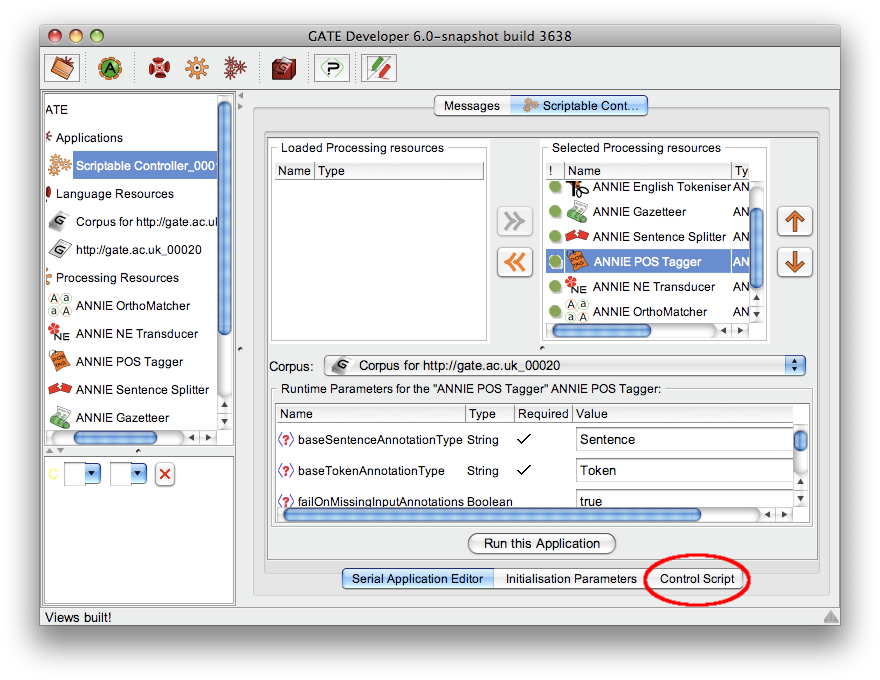
\includegraphics[scale=0.5]{groovy-scriptable-controller.png}
\caption{Accessing the script editor for a scriptable controller}
\label{fig:api:groovy:controller}
\end{center}
\end{figure}

%%%%%%%%%%%%%%%%%%%%%%%%%%%%%%%%%%%%%%%%%%%%%%%%%%%%%%%%%%%%%%%%%%%%%%%%%%%%%
\subsect[sec:api:groovy:utils]{Utility methods}
%%%%%%%%%%%%%%%%%%%%%%%%%%%%%%%%%%%%%%%%%%%%%%%%%%%%%%%%%%%%%%%%%%%%%%%%%%%%%

Loading the Groovy plugin adds some additional methods to several of the core
GATE API classes and interfaces using the Groovy ``mixin'' mechanism.  Any
Groovy code that runs after the plugin has been loaded can make use of these
additional methods, including snippets run in the Groovy console, scripts run
using the Script PR, and any other Groovy code that uses the GATE Embedded API.

The methods that are injected come from two classes.  The
\htlink{http://gate.ac.uk/gate/doc/javadoc/gate/Utils.html}{gate.Utils class}
(part of the core GATE API in gate.jar) defines a number of static methods that
can be used to simplify common tasks such as getting the string covered by an
annotation or annotation set, finding the start or end offset of an annotation
(or set), etc.  These methods do not use any Groovy-specific types, so they are
usable from pure Java code in the usual way as well as being mixed in for use
in Groovy.  Additionally, the class \verb|gate.groovy.GateGroovyMethods| (part
of the Groovy plugin) provides methods that use Groovy types such as closures
and ranges.

The added methods include:
\begin{itemize}
\item Unified access to the start and end offsets of an \verb|Annotation|,
  \verb|AnnotationSet| or \verb|Document|: e.g. \verb|someAnnotation.start()|
  or \verb|anAnnotationSet.end()|
\item Simple access to the \verb|DocumentContent| or string covered by an
  annotation or annotation set: \small{\verb|document.stringFor(anAnnotation)|},
  \small{\verb|document.contentFor(annotationSet)|}
\item Simple access to the length of an annotation or document, either as an
  int (\verb|annotation.length()|) or a long (\verb|annotation.lengthLong()|).
\item A method to construct a \verb|FeatureMap| from any map, to support
  constructions like
  \texttt{def params = [sourceUrl:'http://gate.ac.uk',
    encoding:'UTF-8'].toFeatureMap()}
\item A method to convert an annotation set into a \verb|List| of annotations
  in the order they appear in the document, for iteration in a predictable
  order: \verb|annSet.inDocumentOrder().collect| \verb|{ it.type }|
\item The \verb|each|, \verb|eachWithIndex| and \verb|collect| methods for a
  corpus have been redefined to properly load and unload documents if the
  corpus is stored in a datastore.
\item Various \verb|getAt| methods to support constructions like
  \verb|annotationSet["Token"]| (get all Token annotations from the set),
  \verb|annotationSet[15..20]| (get all annotations between offsets 15 and 20),
  \verb|documentContent[0..10]| (get the document content between offsets 0 and
  10).
\item A \verb|withResource| method for any resource, which calls a closure with
  the resource passed as a parameter, and ensures that the resource is properly
  deleted when the closure completes (analagous to the default Groovy method
  \verb|InputStream.withStream|).
\end{itemize}

For full details, see the source code or javadoc documentation for these two
classes.

%%%%%%%%%%%%%%%%%%%%%%%%%%%%%%%%%%%%%%%%%%%%%%%%%%%%%%%%%%%%%%%%%%%%%%%%%%%%%
\sect{Saving Config Data to gate.xml}
%%%%%%%%%%%%%%%%%%%%%%%%%%%%%%%%%%%%%%%%%%%%%%%%%%%%%%%%%%%%%%%%%%%%%%%%%%%%%

Arbitrary feature/value data items can be saved to the user's {\tt gate.xml}
file via the following API calls:

To get the config data: {\tt Map configData = Gate.getUserConfig()}.

To add config data simply put pairs into the map: {\tt configData.put("my new
config key", "value");}.

To write the config data back to the XML file: {\tt Gate.writeUserConfig();}.

Note that new config data will simply override old values, where the keys are
the same. In this way defaults can be set up by putting their values in the
main gate.xml file, or the site gate.xml file; they can then be overridden by
the user's gate.xml file.


%%%%%%%%%%%%%%%%%%%%%%%%%%%%%%%%%%%%%%%%%%%%%%%%%%%%%%%%%%%%%%%%%%%%%%%%%%%%%
\sect[sec:api:merge]{Annotation merging through the API}
%%%%%%%%%%%%%%%%%%%%%%%%%%%%%%%%%%%%%%%%%%%%%%%%%%%%%%%%%%%%%%%%%%%%%%%%%%%%%


If we have annotations about the same subject on the same document from
different annotators, we may need to merge those annotations to form a unified
annotation. Two approaches for merging annotations are implemented in the API,
via static methods in the class {\bf gate.util.AnnotationMerging}.

The two methods have very similar input and output parameters.  Each of the
methods takes an array of annotation sets, which should be the same annotation
type on the same document from different annotators, as input. A single
feature can also be specified as a parameter (or given as{\em null} if no
feature is to be specified).

The output is a map, the key of which is one merged annotation and the value
of which represents the annotators (in terms of the indices of the array of
annotation sets) who support the annotation. The methods also have a boolean
input parameter to indicate whether or not the annotations from different
annotators are based on the same set of instances, which can be determined by
the static method {\em public boolean
  isSameInstancesForAnnotators(AnnotationSet[] annsA)} in the class {\bf
  gate.util.IaaCalculation}. One instance corresponds to all the annotations
with the same span.  If the annotation sets are based on the same set of
instances, the merging methods will ensure that the merged annotations are on
the same set of instances.

The two methods corresponding to those described for the Annotation Merging
plugin described in Section~\ref{sec:misc-creole:merging}. They are:

\begin{itemize}

\item The Method {\em public static void mergeAnnotation(AnnotationSet[]
    annsArr, String nameFeat, HashMap$<$Annotation,String$>$mergeAnns, int
    numMinK, boolean isTheSameInstances)} merges the annotations stored in the
  array {\em annsArr}. The merged annotation is put into the map {\em
    mergeAnns}, with a key of the merged annotation and value of a string
  containing the indices of elements in the annotation set array {\em annsArr}
  which contain that annotation.  {\em NumMinK} specifies the minimal number
  of the annotators supporting one merged annotation. The boolean parameter
  {\em isTheSameInstances} indicate if or not those annotation sets for
  merging are based on the same instances.

\item Method {\em public static void mergeAnnotationMajority(AnnotationSet[]
    annsArr, String nameFeat, HashMap$<$Annotation, String$>$mergeAnns,
    boolean isTheSameInstances)} selects the annotations which the majority of
  the annotators agree on. The meanings of parameters are the same as those in
  the above method.


\end{itemize}

%%%%%%%%%%%%%%%%%%%%%%%%%%%%%%%%%%%%%%%%%%%%%%%%%%%%%%%%%%%%%%%%%%%%%%%%%%%%%
\sect[sec:api:resourcehelpers]{Using Resource Helpers to Extend the API}
%%%%%%%%%%%%%%%%%%%%%%%%%%%%%%%%%%%%%%%%%%%%%%%%%%%%%%%%%%%%%%%%%%%%%%%%%%%%%
Resource Helpers (see Section \ref{sec:creole-model:tools:resourcehelpers})
are an easy way of adding new features to existing resources within GATE
Developer. Currently most Resource Helpers provide additional ways of loading
or exporting documents, and it would also be useful to have the same features
available via the API. While you could compile embedded code against the plugin
classes or use reflection, this can quickly become difficult to manage, and
rather negates the whole plugin philosophy. Fortunately the Resource Helper
API makes it easy to access these new features from embedded code.

Here is a complete example showing how a GATE document can be exported using
the Resource Helper in the Fast Infoset plugin (see Section
\ref{sec:creole:fastinfoset} for details on Fast Infoset support):

\begin{lstlisting}
// initialise GATE and load the plugin (which creates an autoinstance of the Resource Helper)
Gate.init();
Gate.getCreoleRegister().registerDirectories(
  (new File(Gate.getGateHome(), "plugins/Format_FastInfoset")).toURI()
    .toURL());

// get the autoinstance of the Resource Helper
ResourceHelper rh =
  (ResourceHelper)Gate.getCreoleRegister()
    .getAllInstances("gate.corpora.FastInfosetExporter").iterator()
    .next();

// create a simple test document
Document doc =
  Factory.newDocument("A test of the Resource Handler API access");

// use the Resource Helper to export the document
rh.call("export", doc, new File("resource-handler-test.finf"));
\end{lstlisting}

The comments should make the code fairly self-explanatory, but the main feature
is on line 18 which uses the \lstinline!ResourceHandler.call(String, Resource, Object...)!
method. This essentially allows you to call a named method of the Resource Helper
(in the example ``export''), for a given Resource instance (here we are using a
Document instance), supplying any necessary parameters. This allows you to
access any public method (including static methods) of a Resource Helper that
takes a Resource as it's first parameter.

The only downside to this approach is that there is no compile time checking
that the method you are trying to call actually exists or that the parameters
are of the correct type so testing is important.
